\documentclass[aspectratio=169]{beamer}
\usepackage[backend=bibtex,style=authoryear]{biblatex}
\bibliography{pres3}
\setbeamertemplate{bibliography item}{}
\AtBeginBibliography{\tiny}
\usepackage{lmodern,graphicx,amsthm,amsmath,amssymb,braket,textpos}
\usetheme{focus}
\newcommand{\focus}[1]{\textcolor{blue}{\textbf{#1}}}
\newcommand{\cen}[1]{\begin{center}{#1}\end{center}}

\definecolor{main}{RGB}{40, 40, 40}

\renewcommand{\thefootnote}{}
\renewcommand*\footnoterule{}
\setbeamercolor{footnote}{fg=red}
\setbeamerfont{footnote}{size=\small}

\AtBeginSection[]{
\begin{frame}[noframenumbering]
  \vfill
  \centering
  \begin{beamercolorbox}[sep=8pt,center,rounded=true]{title}
    \usebeamerfont{title}\insertsectionhead\par%
  \end{beamercolorbox}
  \vfill
\end{frame}
}

\title{
\LARGE{Unitary Renormalization Group\\
Solution of the Single-Impurity\\
Anderson model}
}
\subtitle{}
\date{\today}
\author{Abhirup Mukherjee (18IP014)\\[5mm]{Supervisor: Dr. Siddhartha Lal}}

\institute{Department of Physical Sciences\\IISER Kolkata}
\date{\today}
\titlegraphic{
	\vspace*{25pt}
	
\includegraphics[width=3cm]{figures/epqm_logo_mod.jpeg}
	\hspace*{0.5cm}
	
\includegraphics[width=3cm]{figures/dps_logo.jpeg}
}
\begin{document}


\begin{frame}[noframenumbering]
\maketitle
\begin{textblock*}{2cm}(9.4cm,-8.7cm)
	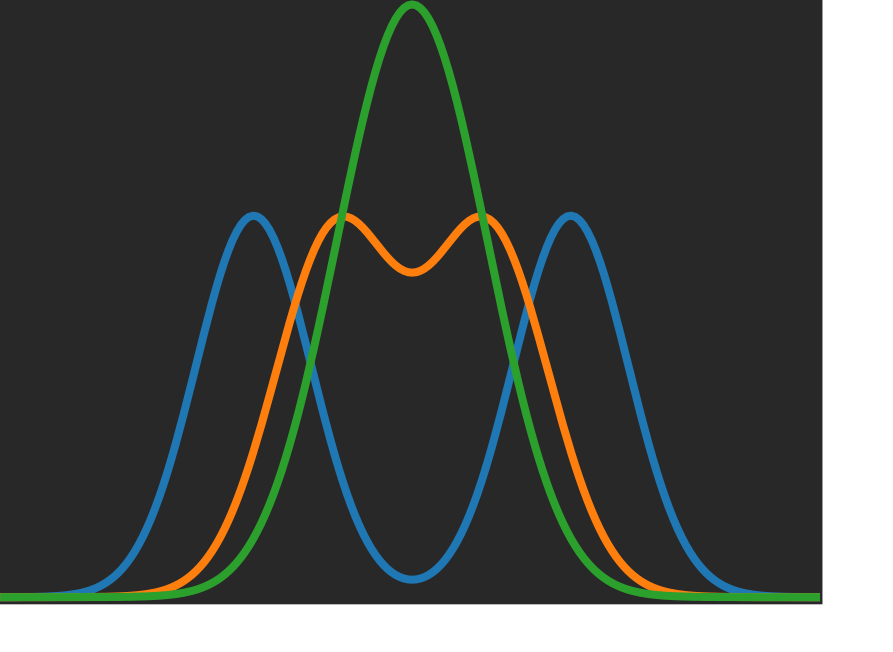
\includegraphics[width=150pt]{figures/title_fig.png}
\end{textblock*}
\end{frame}

\section{The Single-Impurity Anderson Model}
\begin{frame}[noframenumbering]{The Single-Impurity Anderson Model}
\only<+>{
\scalebox{1.38}{
	\hspace*{-10pt}\(\mathcal{H} = \overbrace{\sum_{k\sigma}\epsilon_k \hat n_{k\sigma}}^{\text{conduction}\atop{\text{bath}}} + \overbrace{\sum_{k\sigma}\left[V(k)c^\dagger_{k\sigma}c_{d\sigma} + \text{h.c.}\right]}^\text{hybridisation} + \overbrace{\epsilon_d \sum_\sigma \hat n_{d\sigma}}^{\text{impurity site}\atop{\text{energy}}} + \overbrace{U\hat n_{d\uparrow}\hat n_{d\downarrow}}^\text{d-d repulsion}
\)
}
\begin{minipage}{0.5\textwidth}
\begin{figure}
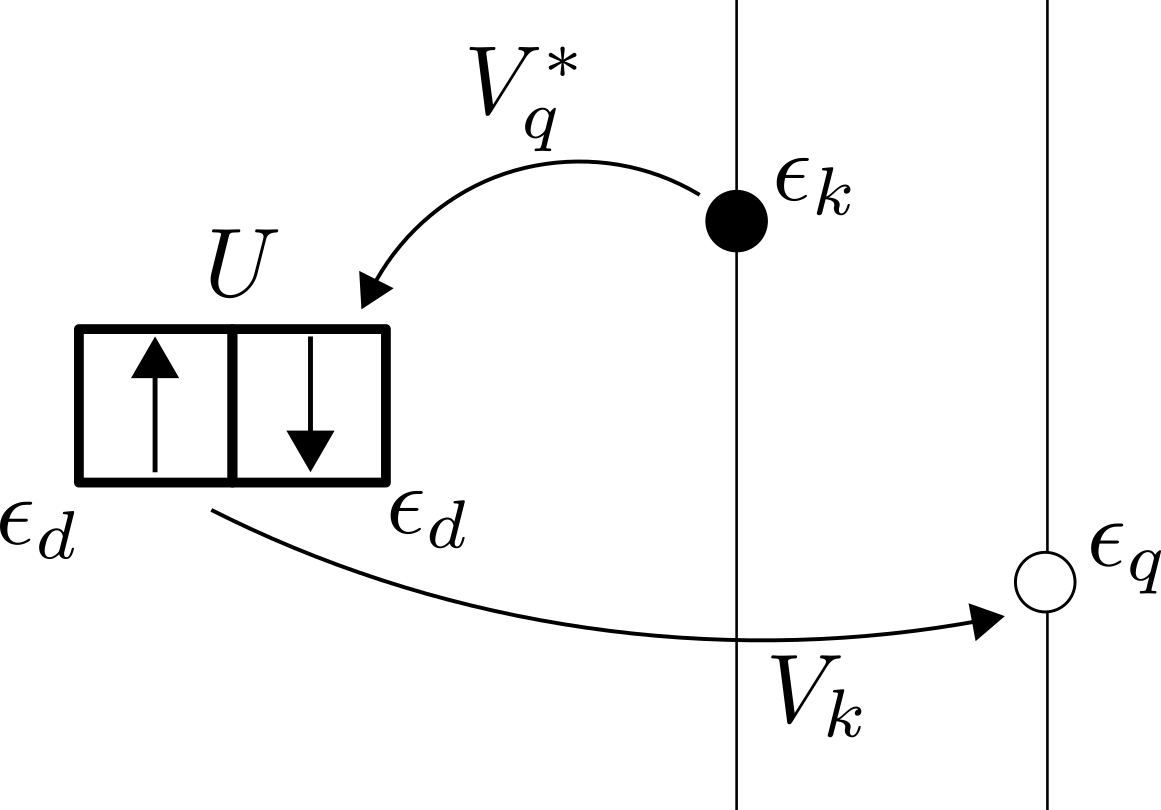
\includegraphics[width=\textwidth]{model_scheme.png}
\end{figure}
\end{minipage}
\begin{minipage}{0.49\textwidth}
\cen{
\LARGE{
	\(\rho(\epsilon) \approx \rho(\epsilon_F)\)\\[20pt]
	\(\Delta = \rho V^2\)\\[20pt]
	\(\epsilon_d = -\frac{1}{2}U\)\large{ (p-h symmetry)}
}
}
\end{minipage}
}
\only<+>{
\begin{tabular}{cl}  
\begin{tabular}{l}
             \parbox{0.5\linewidth}{
\cen{\Large\textbf{NRG Results - Symmetric Model}}
\begin{itemize}
\item the \focus{free-orbital} fixed point (\(U=\Delta=0\)) - unstable
		     \vspace*{10pt}
     \item the \focus{local moment} fixed point (\(U = \infty, \Delta=0\)) - saddle point, and 
		     \vspace*{10pt}
     \item the \focus{strong-coupling} fixed point (\(\Delta=\infty, U = \text{finite}\)) - stable.
\end{itemize}
    }
         \end{tabular}
           &   \begin{tabular}{c}
\includegraphics[scale=0.32]{nrg_fpoints.png}
           \end{tabular}\\
\end{tabular}
\footcite{hrk-nrg}
}
\end{frame}

\section{Some Outstanding Questions}
\begin{frame}[noframenumbering]{Some Outstanding Questions}
  
\begin{itemize}
	\uncover<1->{\item Is it possible to get \focus{non-perturbative scaling equations} for the whole journey?}
	\uncover<2->{\item What is the nature of the strong-coupling fixed point for a \focus{finite system} where \(J \neq \infty\)?
	}
	\uncover<3->{\item Is it possible to show the \focus{transfer of spectral weight} along the flow, possibly by tracking the spectral function?}
	\uncover<4->{\item How does the renormalization affect the \focus{many-particle entanglement} between the electrons?}
	\uncover<5->{\item Are there any interesting \focus{topological aspects} of the fixed points?}
\end{itemize}

\end{frame}

\section{The Unitary Renormalization Group}
\begin{frame}[noframenumbering]{Unitary Renormalization Group: Overview}

	\only<+>{\begin{minipage}{200pt}\cen{\textbf{The Short Version}}Apply \textit{unitary many-body transformations} to the Hamiltonian so as to successively \textit{decouple} high energy states and hence obtain scaling equations.\end{minipage}\begin{minipage}{250pt}\begin{figure}
\def\svgwidth{\columnwidth}
\centering
\scalebox{0.5}{\input{urg_short.pdf_tex}}
\end{figure}\end{minipage}}
\footcite{holography1}
\end{frame}
\begin{frame}[noframenumbering]{URG: Formalism}
\only<+>{\begin{minipage}{200pt}\cen{\large{\textbf{Step 1:}}}Start with the electrons farthest from the Fermi surface. Write the Hamiltonian as \textit{diagonal and off-diagonal terms} in this basis.\end{minipage}\begin{minipage}{300pt}
	\begin{figure}
\def\svgwidth{\columnwidth}
\centering
\input{matrix.pdf_tex}
\end{figure}
\end{minipage}}
\only<+>{\cen{\large{\textbf{Step 2:}}\\Rotate the Hamiltonian to kill the off-diagonal blocks.}
\begin{figure}
\def\svgwidth{\columnwidth}
\centering
\input{rotation.pdf_tex}
\end{figure}
% mention the commutator here
}
\only<+>{\cen{\large{\textbf{Step 3:}}\\Repeat the process with the new blocks.}
\begin{figure}
\def\svgwidth{\columnwidth}
\centering
\input{repeat.pdf_tex}
\end{figure}}
\end{frame}
\begin{frame}[noframenumbering]{URG: Salient Features}
\vspace*{\fill}
\begin{itemize}
	\item Presence of the quantum fluctuation energy scale \(\omega\)
\vspace{10pt}
	\item Presence of finite-valued fixed points
\vspace{10pt}
	\item Spectrum-preserving transformations
\vspace{10pt}
	\item Tractable low-energy effective Hamiltonians
\end{itemize}
\vspace*{\fill}
\end{frame}

\section{Generalized SIAM}
\begin{frame}[noframenumbering]{Model: Generalized SIAM}
\cen{
\scalebox{1.3}{\(H = H_\text{SIAM} + J \vec{S_d}\cdot\vec{s} + K \vec{C_d}\cdot\vec{c}\)}
}
\vspace*{30pt}
\hspace*{\fill}\(\vec{S_d} \equiv \frac{1}{2}\sum_{\alpha\beta}c^\dagger_{d\alpha}\vec{\sigma}_{\alpha\beta}c_{d\beta}\)\hspace*{\fill}\(\vec{s} \equiv \frac{1}{2}\sum_{\alpha\beta}c^\dagger_{0\alpha}\vec{\sigma}_{\alpha\beta}c_{0\beta}\)\hspace*{\fill}
\\
\vspace*{15pt}
\hspace*{\fill}\(\vec{C_d} \equiv \frac{1}{2}\sum_{\alpha\beta}\psi^\dagger_{d\alpha}\vec{\sigma}_{\alpha\beta}\psi_{d\beta}\)\hspace*{\fill}\(\vec{c} \equiv \frac{1}{2}\sum_{\alpha\beta}\psi^\dagger_{0\alpha}\vec{\sigma}_{\alpha\beta}\psi_{0\beta}\)\hspace*{\fill}
\\
\vspace*{15pt}
\hspace*{\fill}\(\vec{\psi}_d \equiv \begin{pmatrix} c_{d \uparrow} \\ c^\dagger_{d \downarrow}\end{pmatrix} \)\hspace*{\fill}\(\vec{\psi}_0 \equiv \sum_k \begin{pmatrix} c_{k \uparrow} \\ c^\dagger_{k \downarrow}\end{pmatrix}\)\hspace*{\fill}
\footcite{Schrieffer_Wolff}
\end{frame}

\section{RG Equations, Their Features and Fixed Points}
\begin{frame}[noframenumbering]{RG Equations}
\[
\Delta U = 4|V|^2 \left[\frac{1}{\omega - \frac{1}{2}D + \frac{U}{2} + \frac{1}{2}J}  - \frac{1}{\omega - \frac{1}{2}D - \frac{U}{2} + \frac{1}{2}K}\right] + \sum_{k<\Lambda_j} \frac{3}{4}\frac{K^2 - J^2}{\omega - \frac{1}{2}D + \frac{1}{4}J + \frac{1}{4}K}
\]

\[
	\hspace*{-10pt}\Delta V = \frac{V K}{16}\left(\frac{1}{\omega - \frac{1}{2}D - \frac{U}{2} + \frac{1}{2}K} + \frac{1}{\omega - \frac{1}{2}D + \frac{1}{4}J + \frac{1}{4}K} \right) - \frac{3VJ}{4}\left( \frac{1}{\omega - \frac{1}{2}D + \frac{U}{2} + \frac{1}{2}J} + \frac{1}{\omega - \frac{1}{2}D + \frac{1}{4}J + \frac{1}{4}K} \right)
\]

\[
\Delta J = - J^2\left(\omega - \frac{1}{2}D + \frac{1}{4}J + \frac{1}{4}K\right)^{-1}
\]

\[
\Delta K = - K^2\left(\omega - \frac{1}{2}D + \frac{1}{4}J + \frac{1}{4}K\right)^{-1}
\]
\end{frame}

\begin{frame}{Passage to Poor Man's Scaling Results}
\begin{minipage}{0.35\textwidth}
\begin{itemize}
	\item \(J=0, K=0\)
	\item \(\omega = -\frac{D}{2}\)
	\item \(U = -\frac{\epsilon_d}{2} \ll D\)
\end{itemize}
\end{minipage}
\begin{minipage}{0.2\textwidth}
	{\LARGE \[\longrightarrow\]}
\end{minipage}
\begin{minipage}{0.35\textwidth}
	\centering
	\Large \(\delta U = \delta V = 0\)
\end{minipage}

\vspace*{30pt}
\begin{minipage}{0.35\textwidth}
\begin{itemize}
	\item \(J=0, K=0\)
	\item \(\omega = -\frac{D}{2}\)
	\item \(U \gg D \gg \epsilon_d\)
\end{itemize}
\end{minipage}
\begin{minipage}{0.2\textwidth}
	{\LARGE \[\longrightarrow\]}
\end{minipage}
\begin{minipage}{0.35\textwidth}
	\centering
	\Large\(\delta U = \delta V = 0\)\\[10pt]
	\(\delta \epsilon_d = \frac{\Delta}{\pi}\delta \ln{D}\)

\end{minipage}
\end{frame}

\begin{frame}{Fixed Points}
\begin{minipage}{0.6\textwidth}
	\begin{itemize}
		\item \(J=K=0 \longrightarrow \Delta V = 0\)
			\vspace*{20pt}
		\item \(J,K,V=0^+ \longrightarrow \left(V^*, J^*, K^*\right)=\text{large}, U^*=0\)
			\begin{itemize}
				\item \focus{strong-coupling fixed point}
			\end{itemize}
			\vspace*{20pt}
		\item \(J=K=V=0 \longrightarrow \text{all couplings marginal}\)
			\begin{itemize}
				\item line of fixed points on y-axis
			\end{itemize}
			\vspace*{20pt}
		\item \(U=0^+ \longrightarrow \text{\focus{local moment fixed point}}\)
			\begin{itemize}
				\item ground-state is a decoupled impurity spin
			\end{itemize}
	\end{itemize}
\end{minipage}
\begin{minipage}{0.38\textwidth}
	\centering
	\includegraphics[width=\textwidth]{figures/nrg_fpoints.png}
\end{minipage}
	
\end{frame}
\begin{frame}[noframenumbering]{Results: \(U>0, J>K\)}
\begin{minipage}{0.6\textwidth}
\cen{
	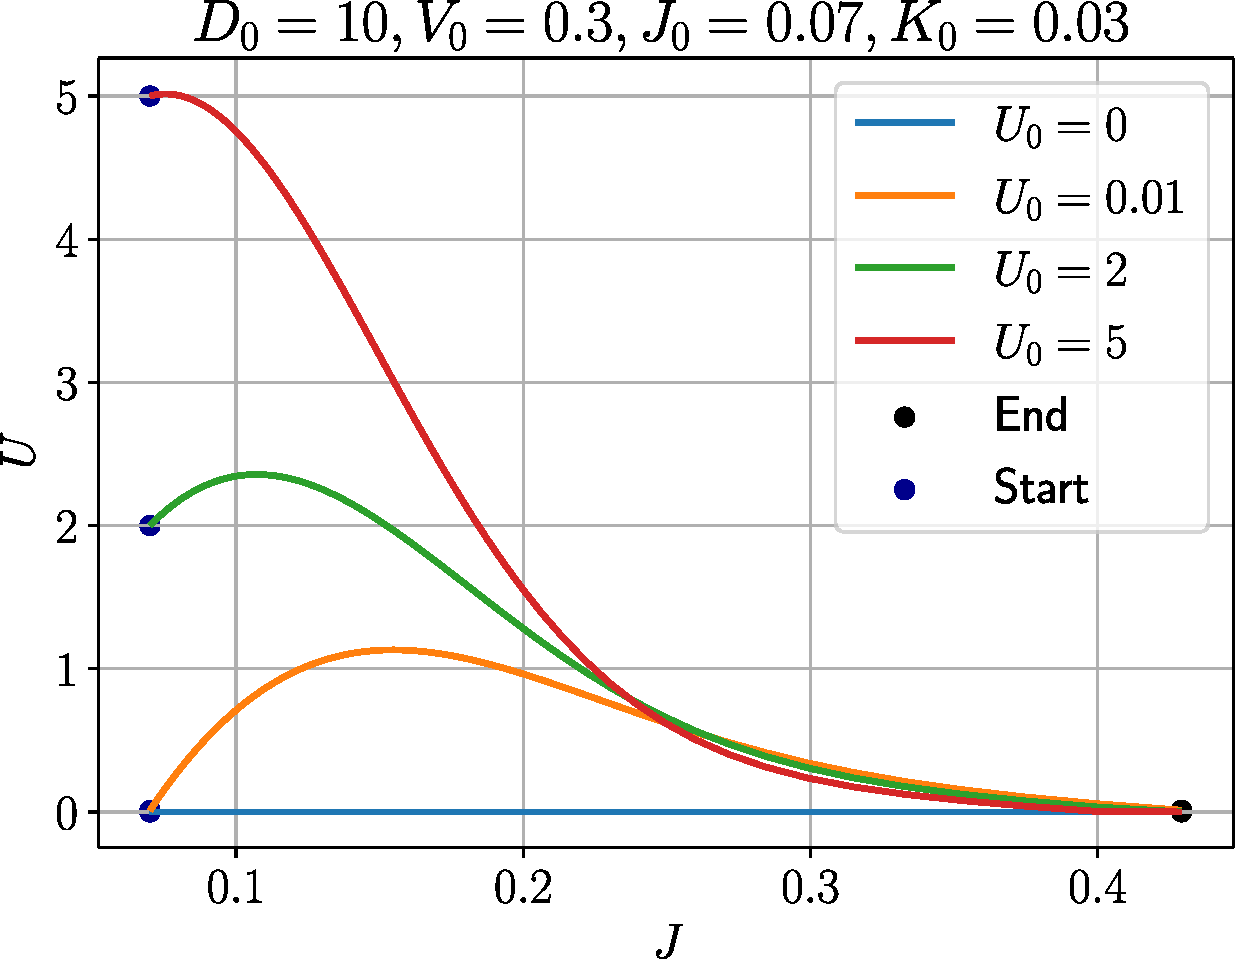
\includegraphics[width=\textwidth]{figures/UvsJ.pdf}
}
\end{minipage}
\begin{minipage}{0.39\textwidth}
\cen{
	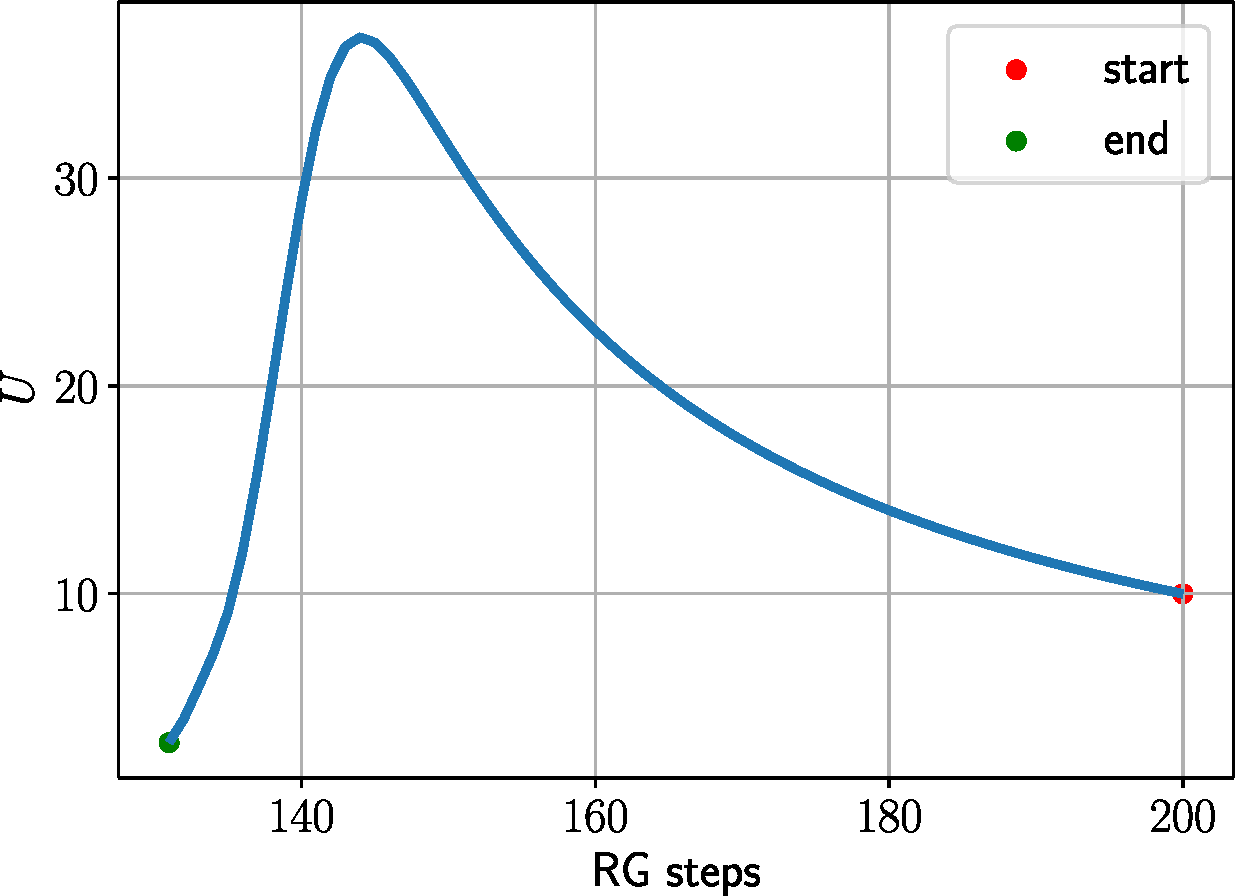
\includegraphics[width=0.95\textwidth]{figures/U_vs_count.pdf}
	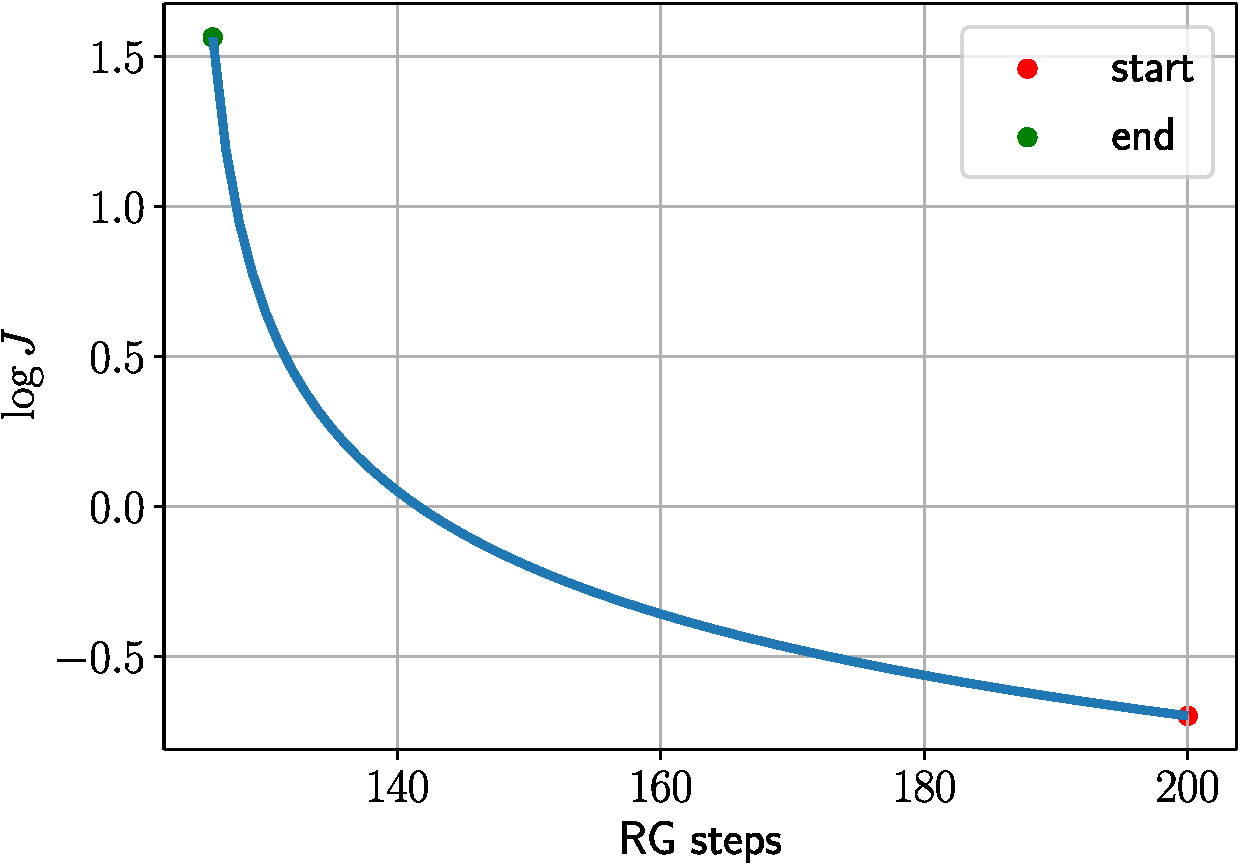
\includegraphics[width=0.95\textwidth]{figures/J_vs_count.pdf}
}
\end{minipage}
\end{frame}


\begin{frame}[noframenumbering]{Results: \(U<0, J<K\)}
	\vspace*{30pt}
\cen{
	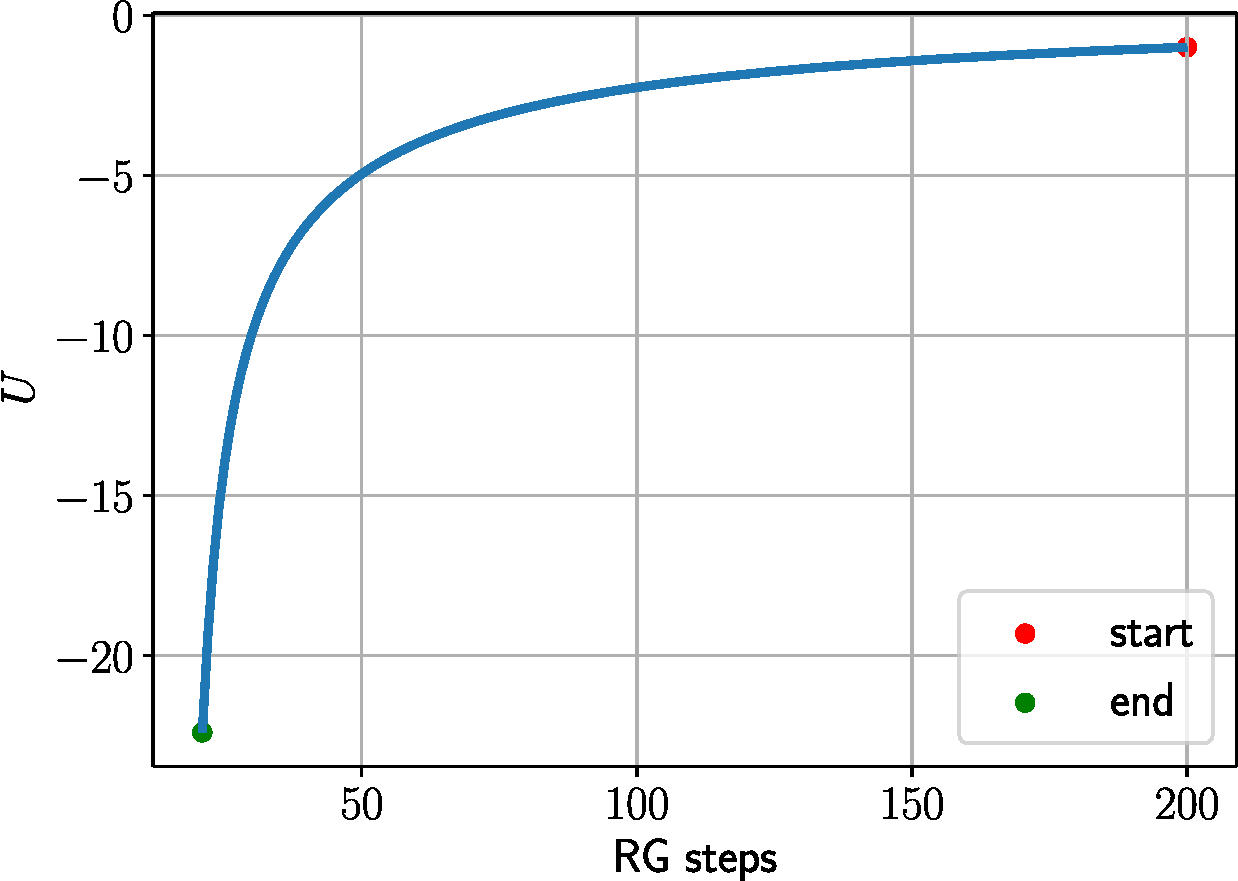
\includegraphics[width=0.49\textwidth]{figures/U_vs_count_neg.pdf}
	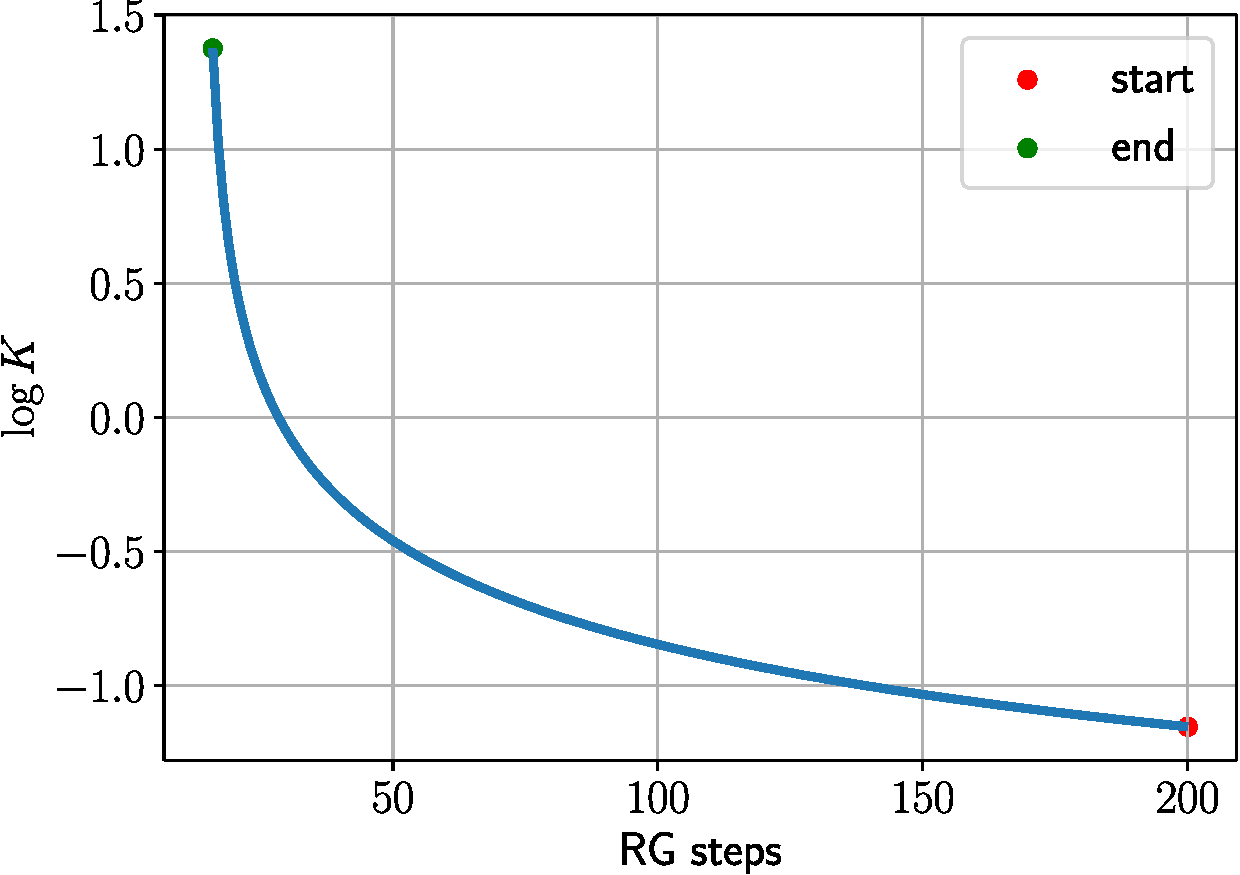
\includegraphics[width=0.49\textwidth]{figures/K_vs_count_neg.pdf}
}
\end{frame}

\section{Low energy effective theory and ground state wavefunctions}
\begin{frame}[noframenumbering]{Results: Phase Diagram}
\cen{
	\hspace*{-50pt}\def\svgwidth{0.8\columnwidth}
	\input{phases-V-pres.pdf_tex}
	% 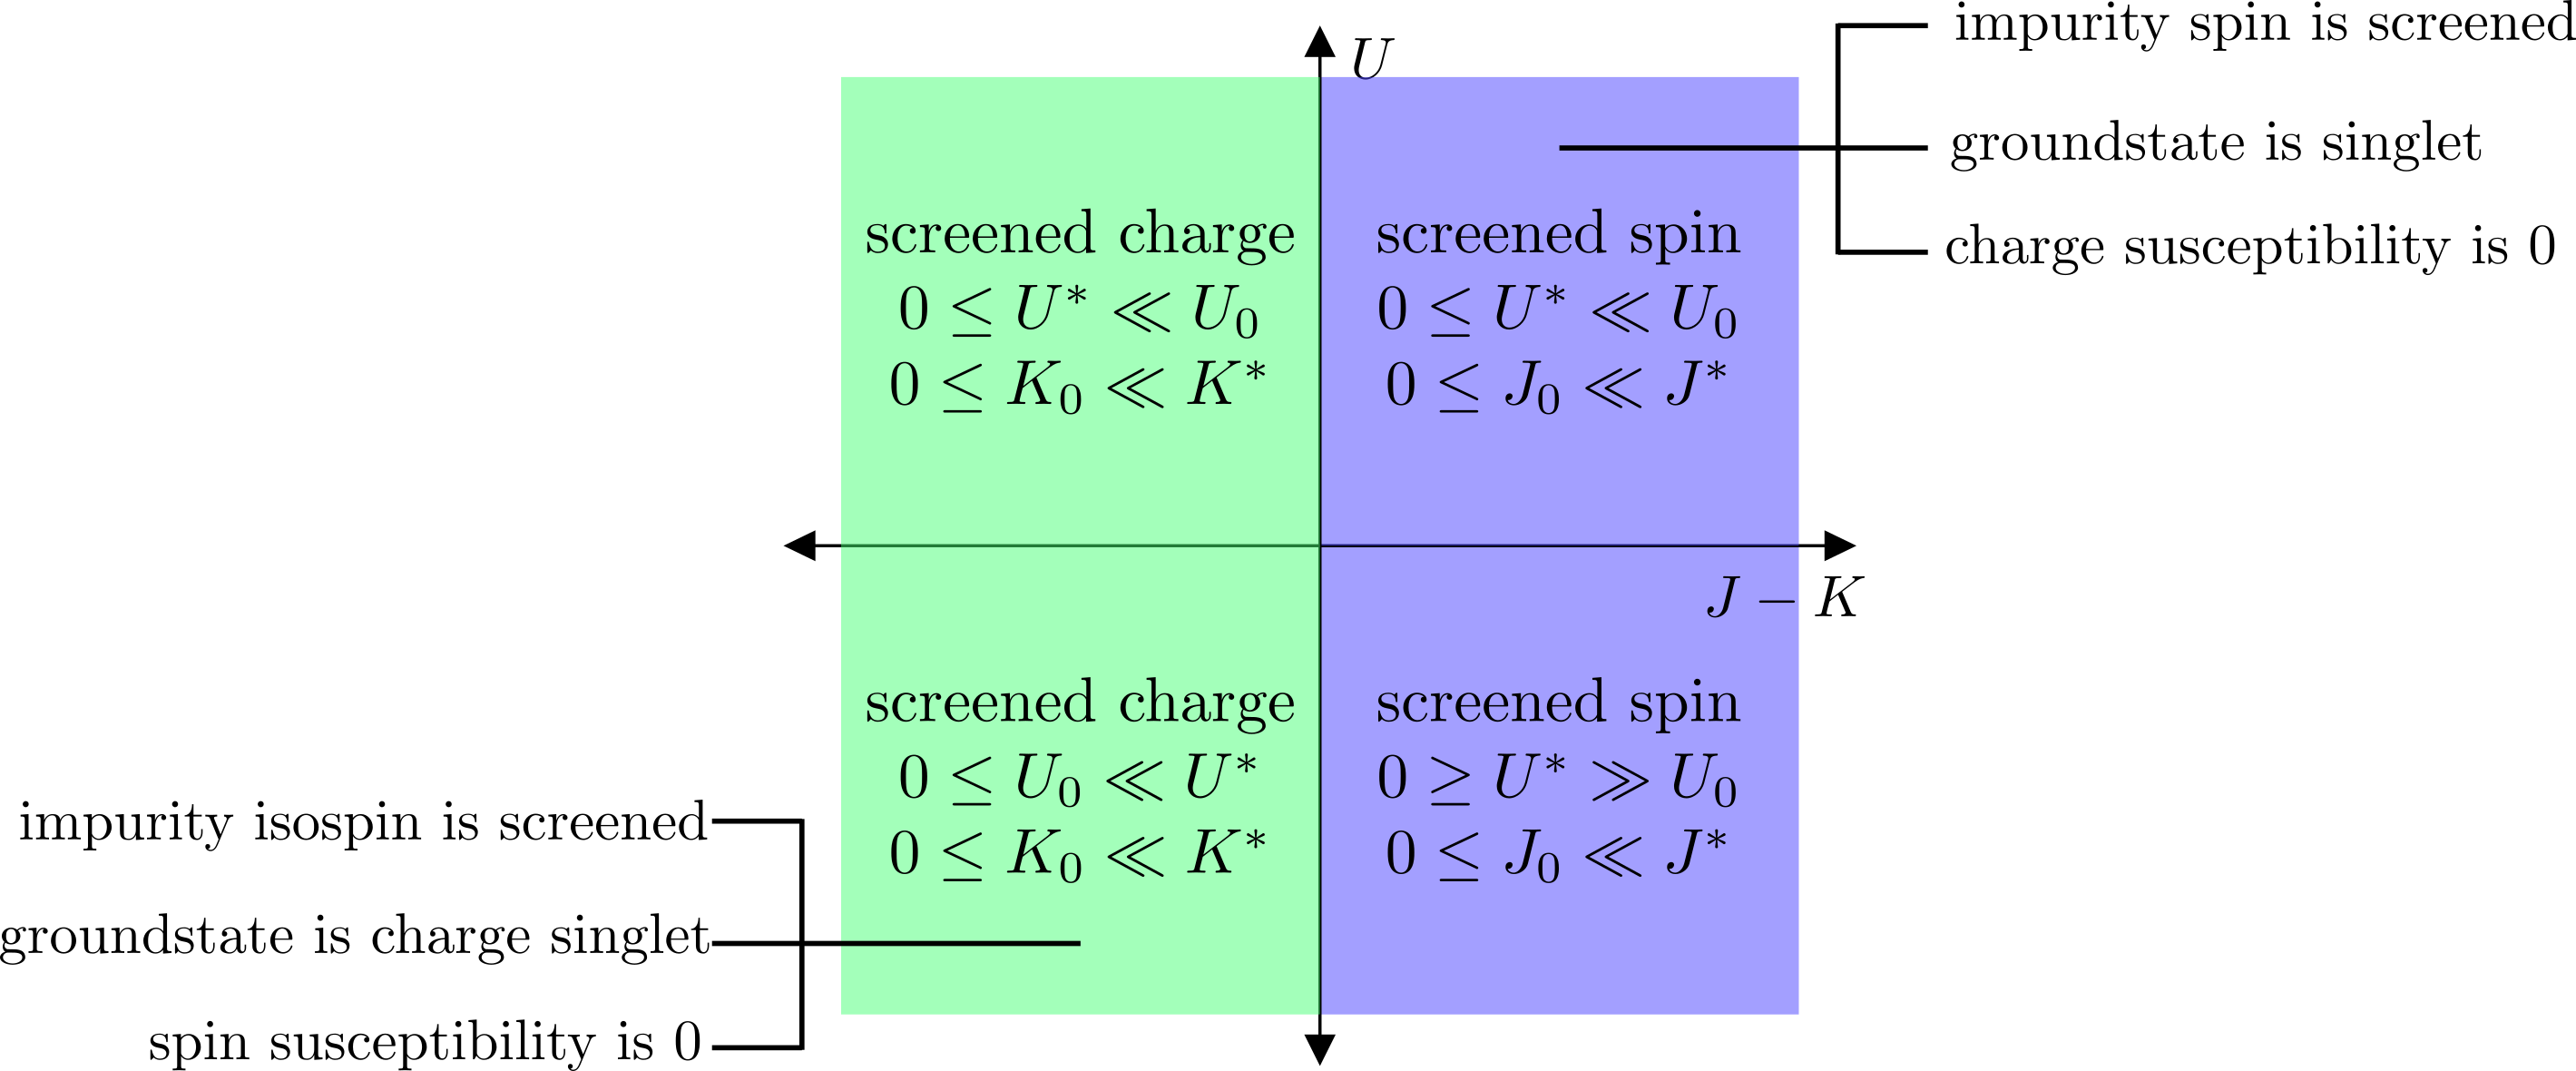
\includegraphics[width=0.99\textwidth]{figures/phases_V_pres.png}
}
\end{frame}


\begin{frame}[noframenumbering]{Results: Effective Zero-mode Hamiltonian}
	\vspace*{-30pt}
	\[H_{IR} = \epsilon_d^* \left( \hat n_{1 \uparrow} - \hat n_{1 \downarrow} \right) ^2 + V^*\sqrt{N^*}\sum_{\sigma}\left(c^\dagger_{1\sigma}c_{2\sigma} + \text{h.c.} \right) + J^*N^*\vec{S_1}\cdot\vec{S_2} + K^*N^*\vec{C_1}\cdot\vec{C_2}\]
\hspace*{-15pt}
	\begin{minipage}{0.5\textwidth}
	{\centering
	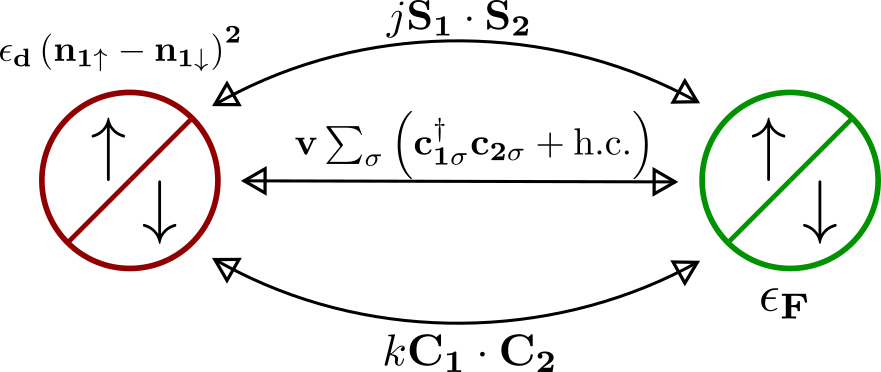
\includegraphics[width=\textwidth]{figures/two_site_problem.png}}
\end{minipage}
\hspace*{25pt}
\begin{minipage}{0.45\textwidth}
	{\centering
	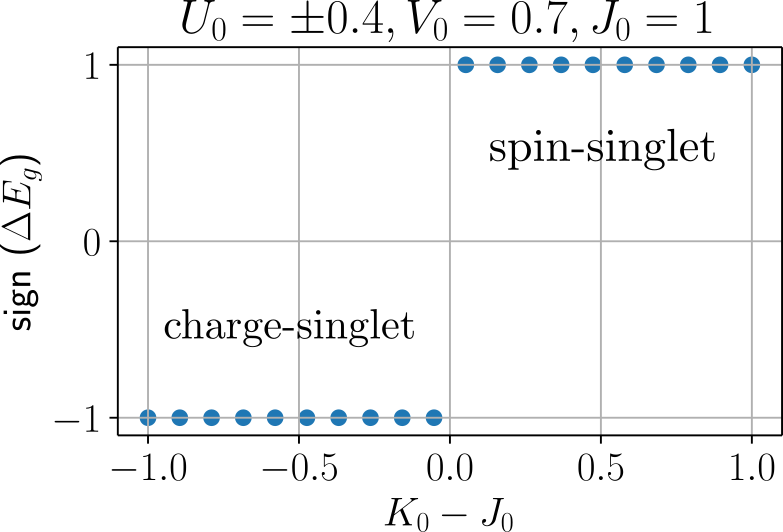
\includegraphics[width=\textwidth]{figures/gstate_state.png}}
\end{minipage}

\footcite{wilson,hrk-nrg,taraphder}

\end{frame}

\begin{frame}[noframenumbering]{Results: Ground State}
\begin{minipage}{0.65\textwidth}
	\[J > K, U>0\]
\vspace*{-10pt}
	\[\ket{\Psi}_\text{GS} = c_-^s\left[\ket{\uparrow, \Downarrow} - \ket{\downarrow, \Uparrow}\right] + c_-^c\left[\ket{\uparrow, \Downarrow} + \ket{\downarrow, \Uparrow}\right]\]

\vspace*{10pt}
\begin{minipage}{0.65\textwidth}
\begin{figure}[htpb]
	\centering
	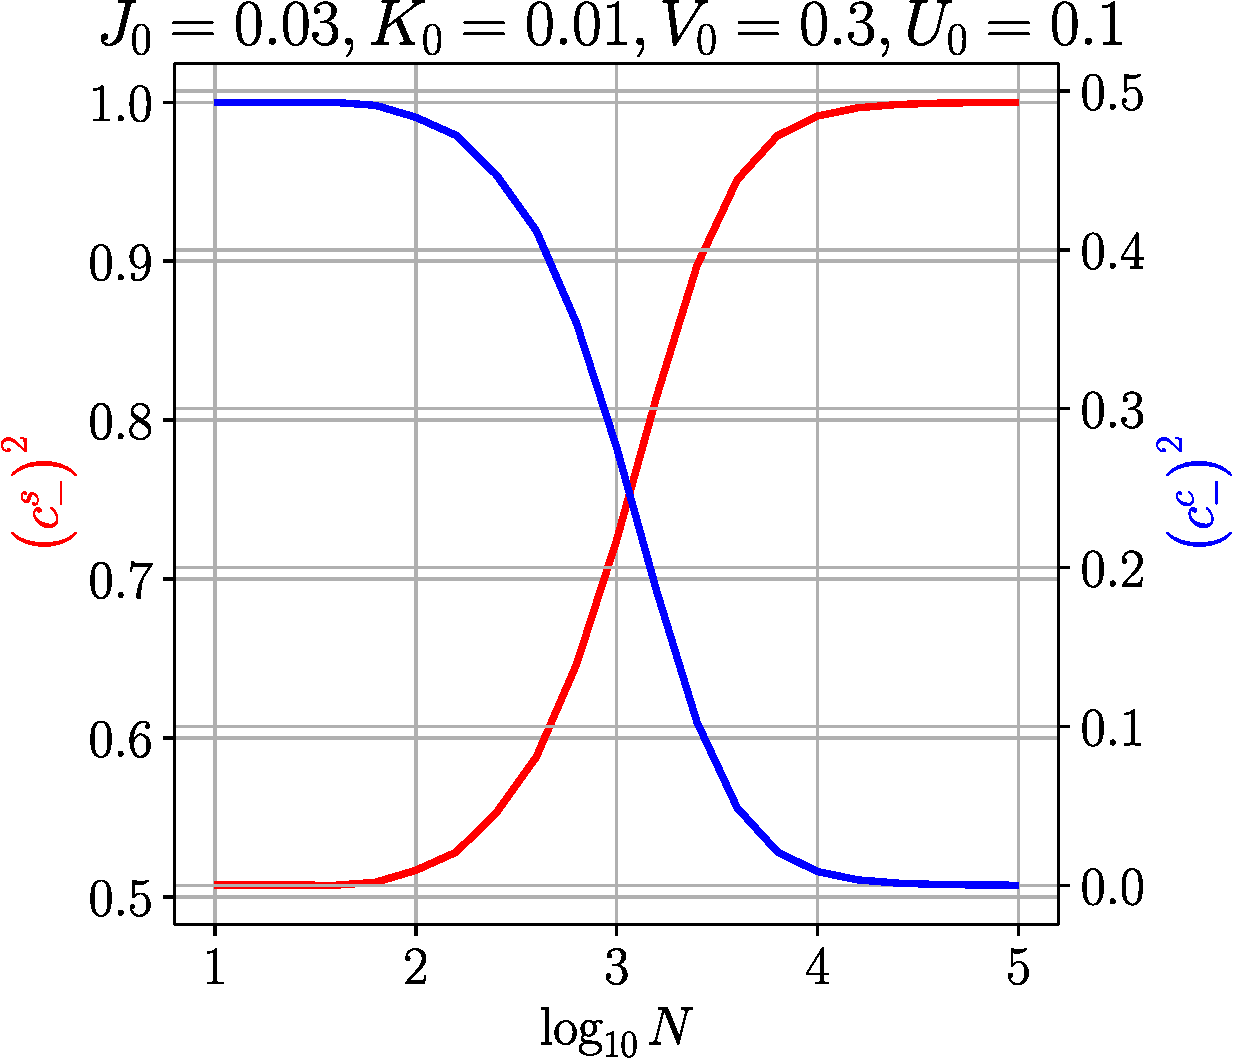
\includegraphics[width=0.8\textwidth]{figures/cscc_q1.pdf}
\end{figure}
\end{minipage}
\begin{minipage}{0.3\textwidth}
	\[ c_-^s \to 1\]
	\[ c_-^c \to 0\]
\end{minipage}
\[\ket{\Psi}_\text{GS} \sim \left[\ket{\uparrow, \Downarrow} - \ket{\downarrow, \Uparrow}\right]\]
\end{minipage}
\vline
\begin{minipage}{0.34\textwidth}
\[J < K, U<0\]
\[\ket{\Psi}_\text{GS} = \left[\ket{\uparrow_c, \Downarrow_c} - \ket{\downarrow_c, \Uparrow_c}\right]\]
\vspace*{0.6\textheight}
\end{minipage}
\end{frame}

\section{Impurity Susceptibilities and Impurity spectral function}
\begin{frame}[noframenumbering]{Results: Spin Susceptibility}
	\vspace*{-20pt}
	\[\chi_s = \lim_{B \to 0} \frac{\partial{m}}{\partial{B}}\]
\cen{
	\hspace*{-20pt}
	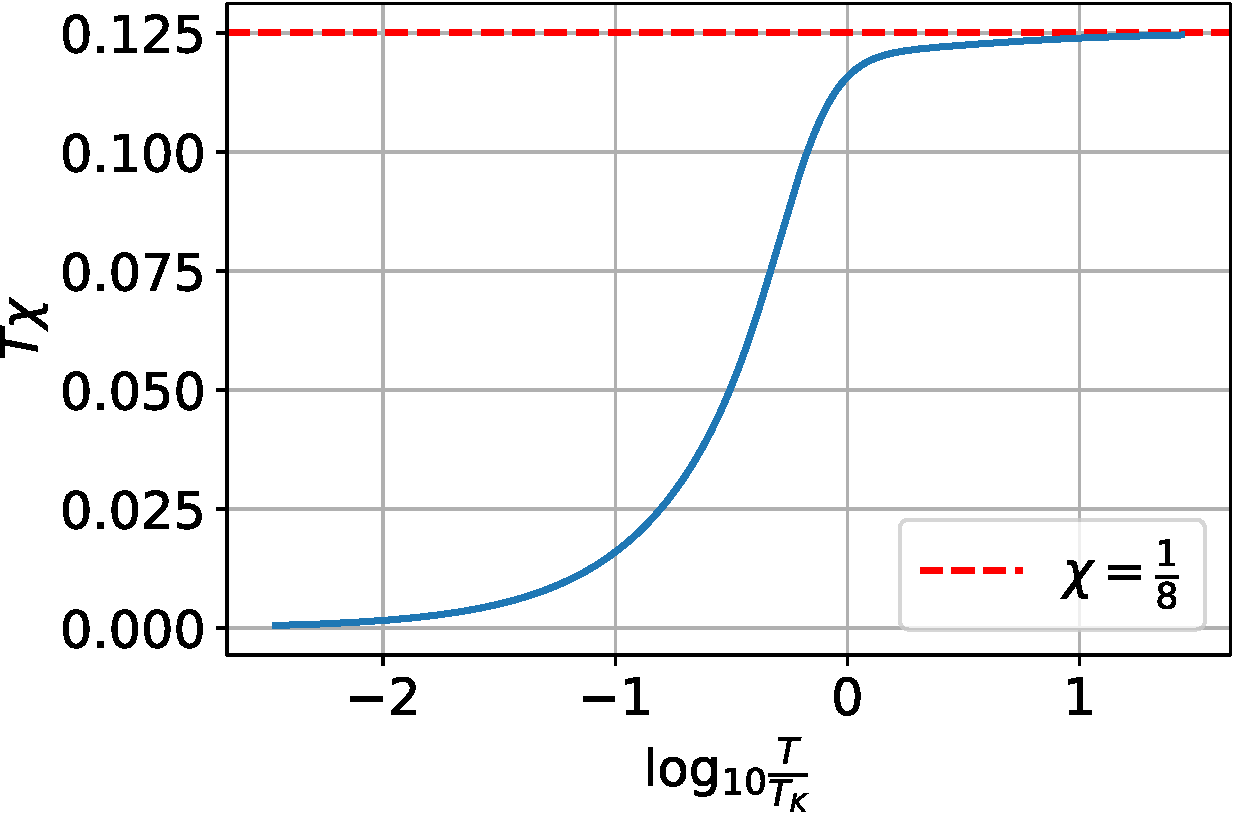
\includegraphics[width=0.48\textwidth]{figures/chi_T.pdf}
	\hspace*{25pt}
	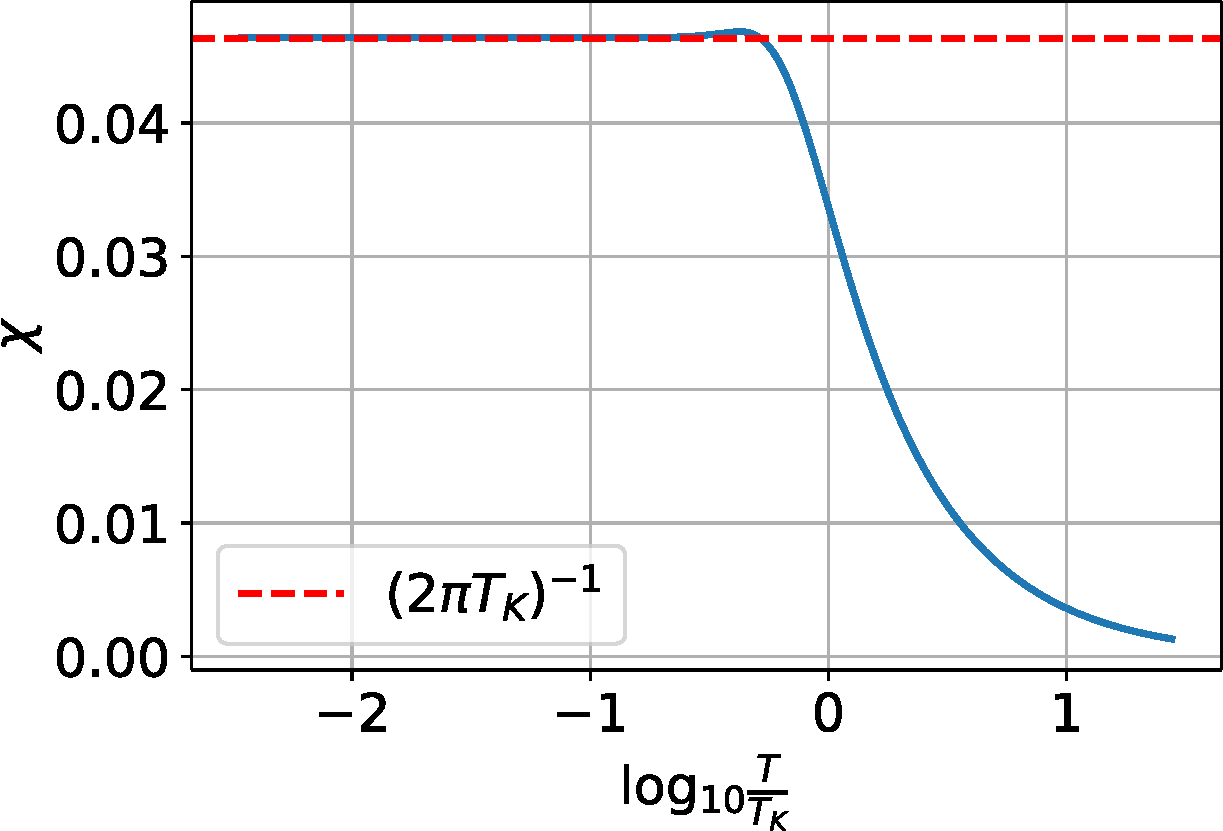
\includegraphics[width=0.48\textwidth]{figures/chi.pdf}
}
\hspace*{20pt}\large{\(
\left(\chi\times T\right)\left( T \to 0 \right) = \frac{1}{2j} \hspace*{\fill} T_K \equiv \frac{2N^*}{\pi}\left(D^* - 2\omega\right)\hspace*{\fill} \chi \left( T \to \infty \right) = \frac{1}{8}\)}

\footcite{wilson, hrk-nrg}
\end{frame}

\begin{frame}[noframenumbering]{Results: Charge Susceptibility}
	\vspace*{-15pt}
	\[\chi_c = \lim_{\mu \to 0} \frac{\partial{N}}{\partial{\mu}}\]
\cen{
	\hspace*{-20pt}
	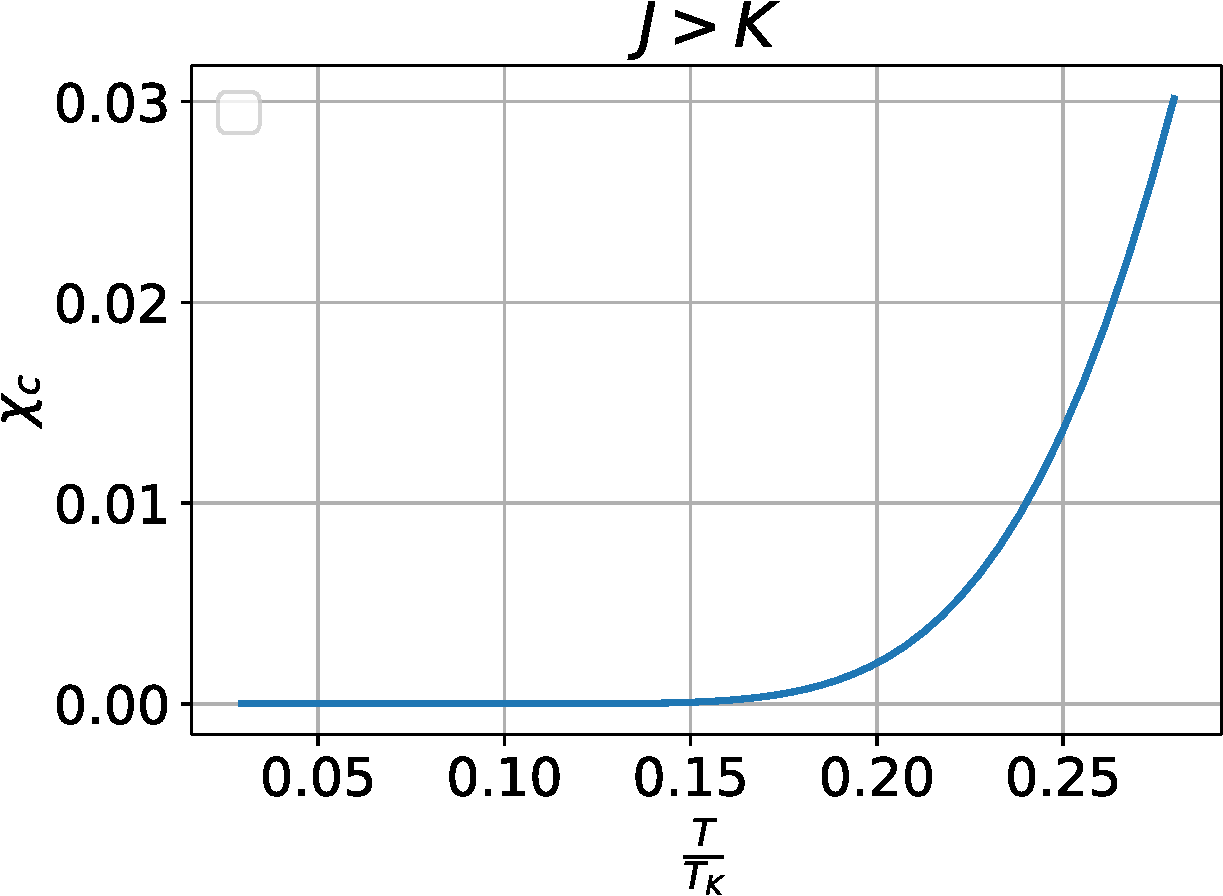
\includegraphics[width=0.48\textwidth]{figures/chi_c.pdf}
	\hspace*{25pt}
	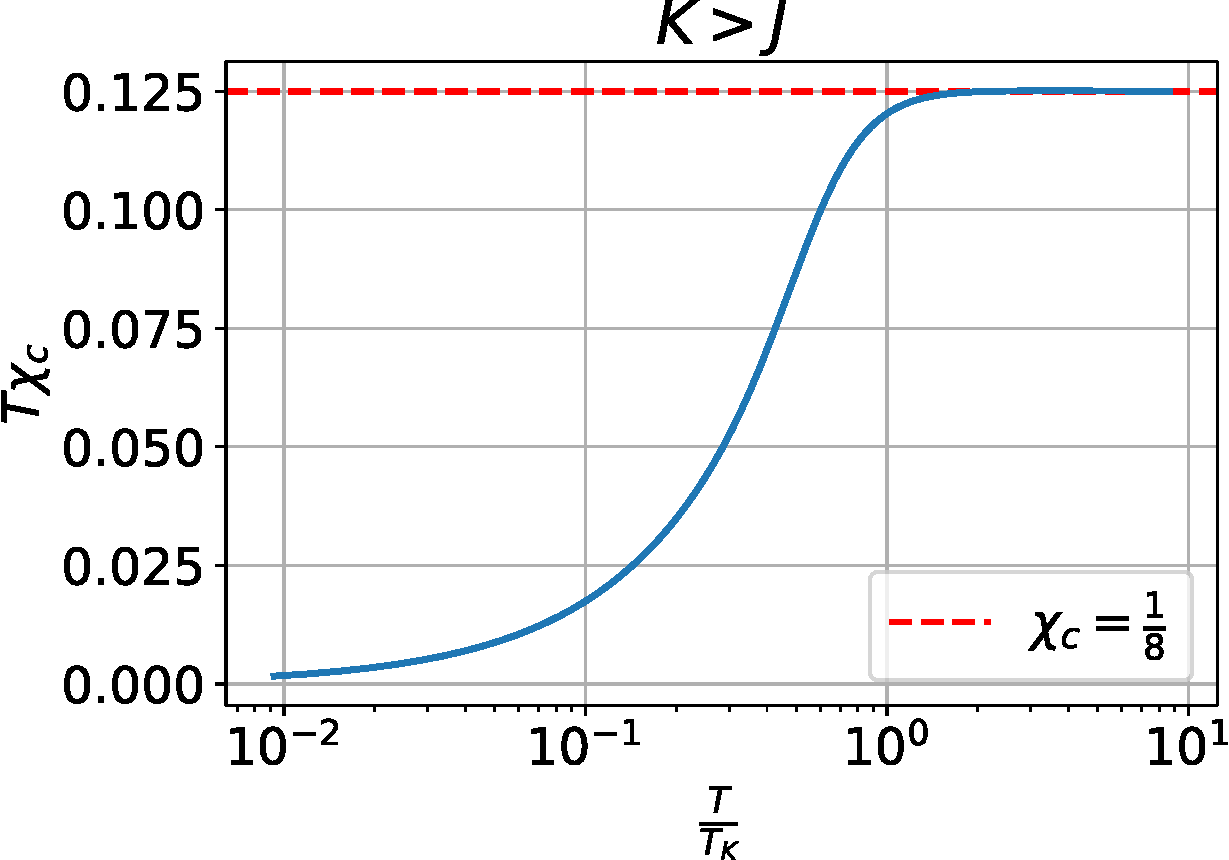
\includegraphics[width=0.48\textwidth]{figures/T_chi_c.pdf}
}
\large{\(
\left(\chi_c\times T\right)\left(T \to 0\right)\big\vert_{K>J} = \frac{1}{2k} \quad\quad\quad \left(\chi_c\times T\right)\left(T \to 0\right)\big\vert_{J>K} = 0 \quad\quad\quad \chi \left( T \to \infty \right) = \frac{1}{8}\)}

\footcite{taraphder,charge-kondo-Zitko}
\end{frame}

\begin{frame}[noframenumbering]{Results: Impurity Spectral Function}
	\(\mathcal{A(\omega)} = -\frac{1}{\pi}\text{Im }\left[G_{d d}^\sigma\left( \omega \right) \right]\) \hspace*{\fill} \(G_{d d}^\sigma\left(t\right) = -i\theta(t)\left<\left\{ c_{d\sigma}(t), c^\dagger_{d\sigma} \right\}\right>\)
\cen{
	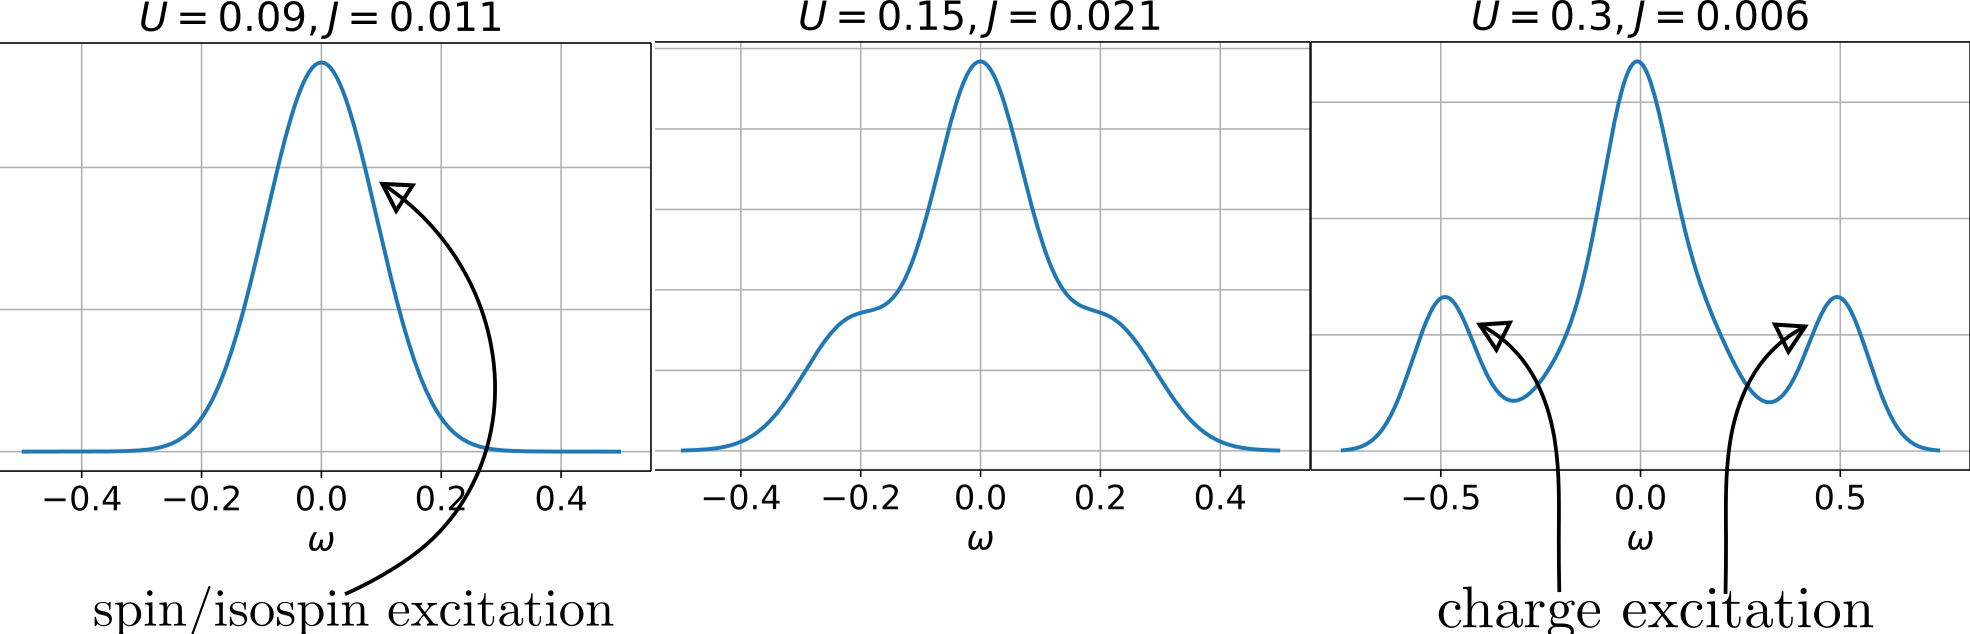
\includegraphics[width=\textwidth]{figures/spec_func_merged_2.png}
}
\footcite{hewson,bulla_costi_nrg}
\end{frame}

\begin{frame}[noframenumbering]{Results: Spectral Function Renormalization}
	\(\mathcal{A(\omega)} = -\frac{1}{\pi}\text{Im }\left[G_{d d}^\sigma\left( \omega \right) \right]\) \hspace*{\fill} \(G_{d d}^\sigma\left(t\right) = -i\theta(t)\left<\left\{ c_{d\sigma}(t), c^\dagger_{d\sigma} \right\}\right>\)
\cen{
	\includegraphics[width=0.47\textwidth]{figures/spec_func_journey_one_marked.pdf}\hspace*{\fill}\includegraphics[width=0.45\textwidth]{figures/spec_func_journey_three_marked.pdf}
}
\end{frame}

\section{Entanglement measures and Topological Features of low energy theory}
\begin{frame}[noframenumbering]{Results: Kondo Cloud Hamiltonian}
	\vspace*{-10pt}
	\[H^*(\text{d, cloud}) \xrightarrow{\text{solve for bath Hamiltonian}} H^*_\text{cloud}\] 
	\[H^*_\text{cloud} = \overbrace{H^*_0}^\text{kinetic energy} + \overbrace{\sum_{kk^\prime\sigma\sigma^\prime}f_{kk^\prime}\hat n_{k\sigma}\hat n_{k^\prime\sigma^\prime}}^\text{Fermi liquid-type interaction} + \overbrace{\sum_{kk^\prime qq^\prime}F_{kk^\prime qq^\prime}c^\dagger_{k \uparrow}c^\dagger_{k^\prime \downarrow} c_{q \uparrow}c_{q^\prime \downarrow}}^\text{non-Fermi liquid-type interaction}\]
\begin{figure}[htpb]
	\centering
	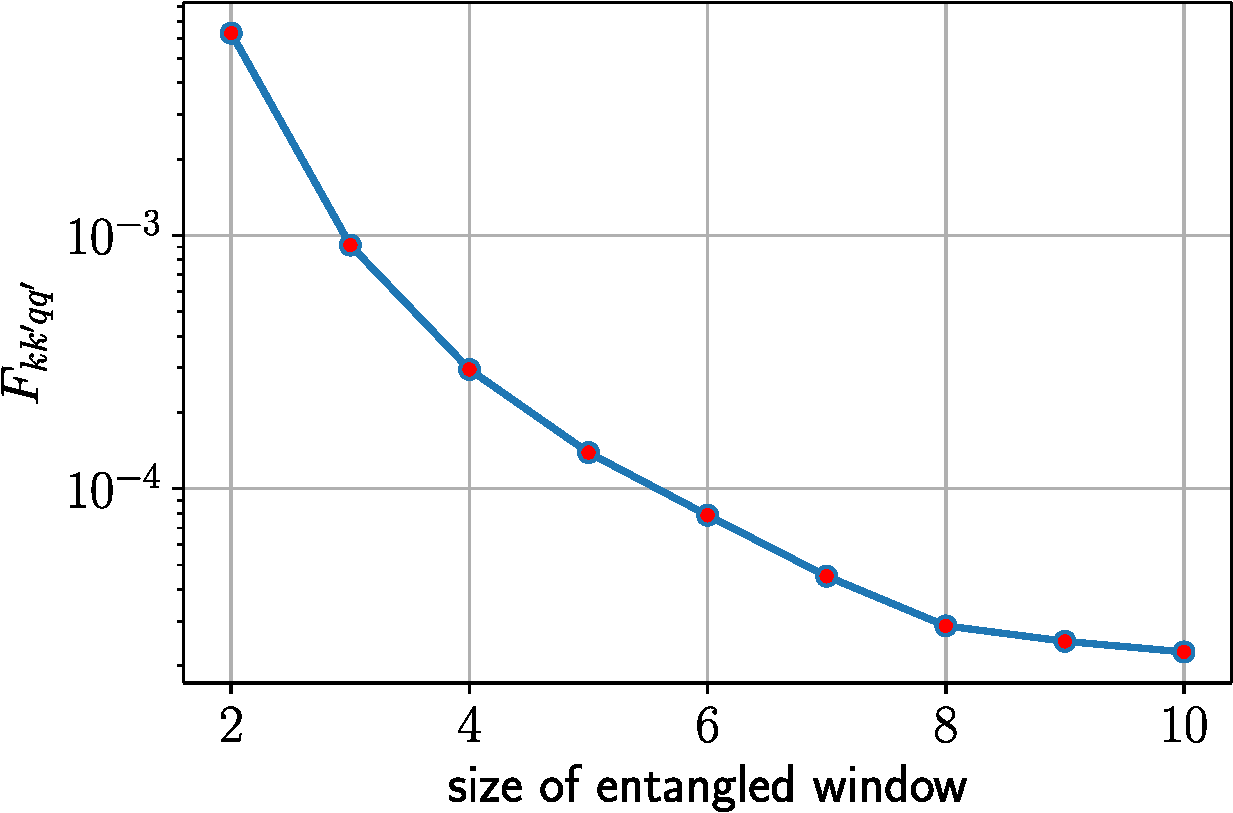
\includegraphics[width=0.45\textwidth]{figures/Fkkqq.pdf}
\end{figure}
\end{frame}

\begin{frame}[noframenumbering]{Results: Reverse RG: Overview}
	\vspace*{\fill}
	\begin{figure}[htpb]
		\centering
		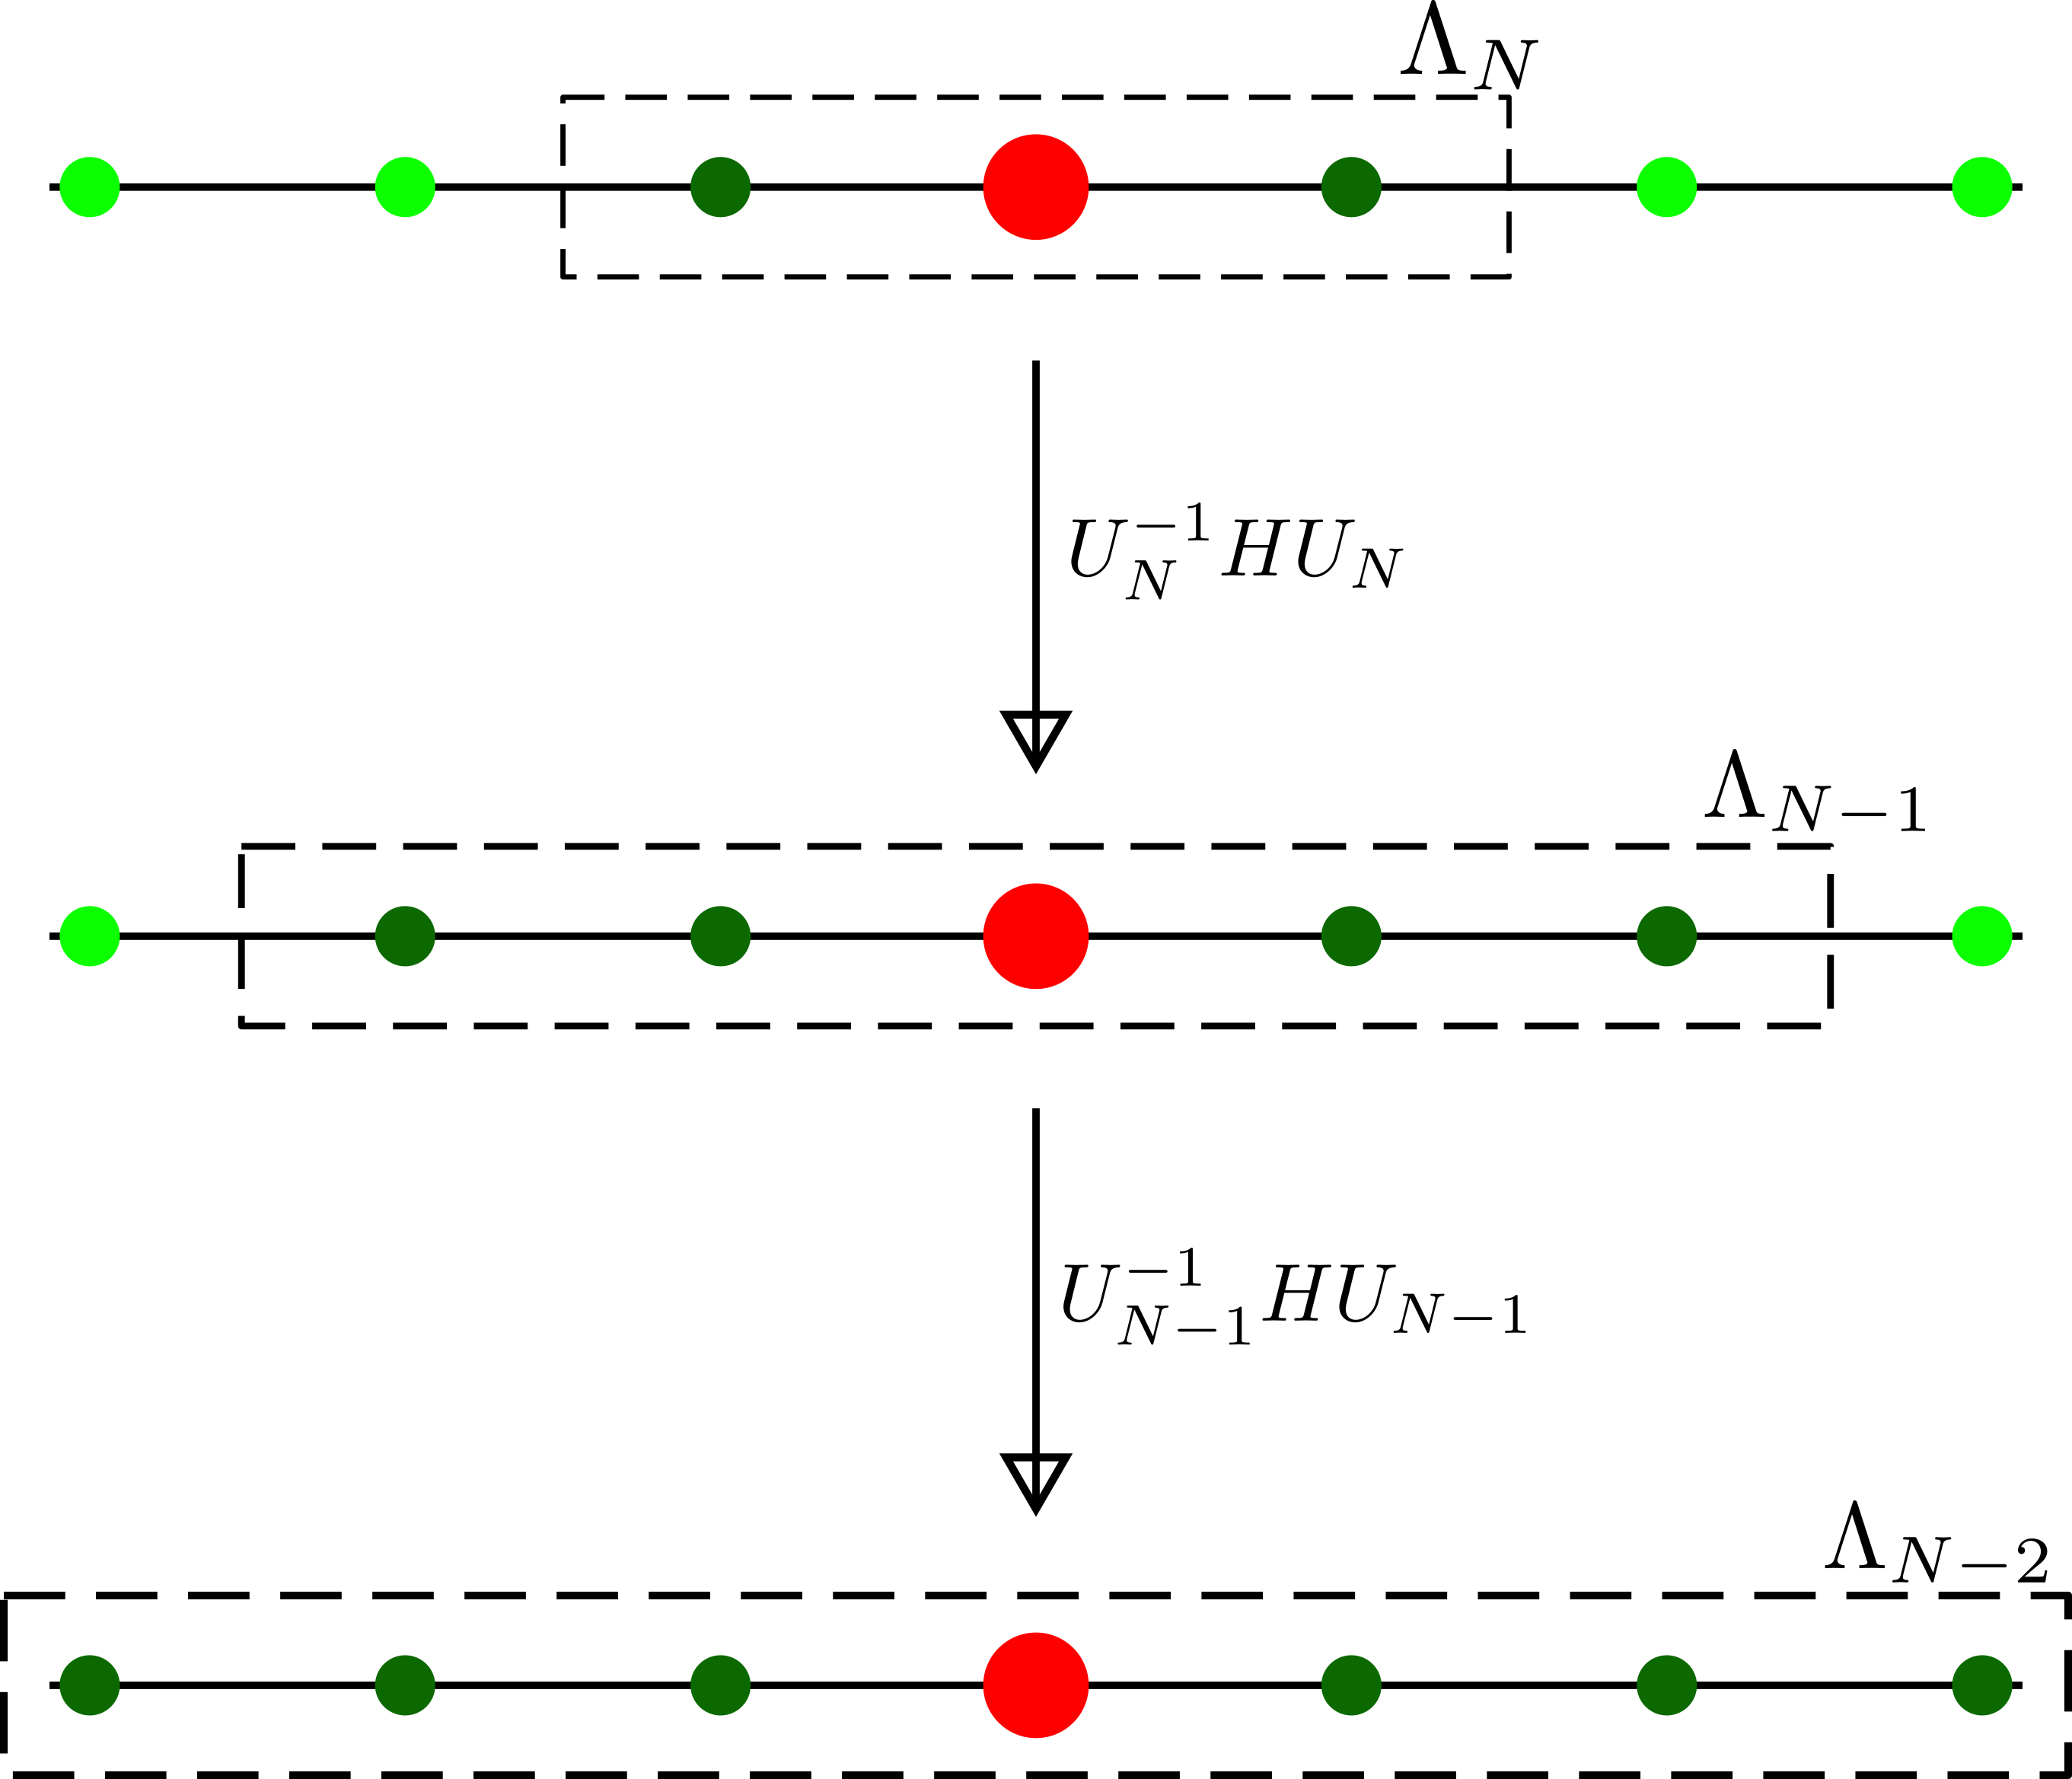
\includegraphics[width=0.5\textwidth]{figures/reverse-rg.png}
		\hspace*{\fill}
		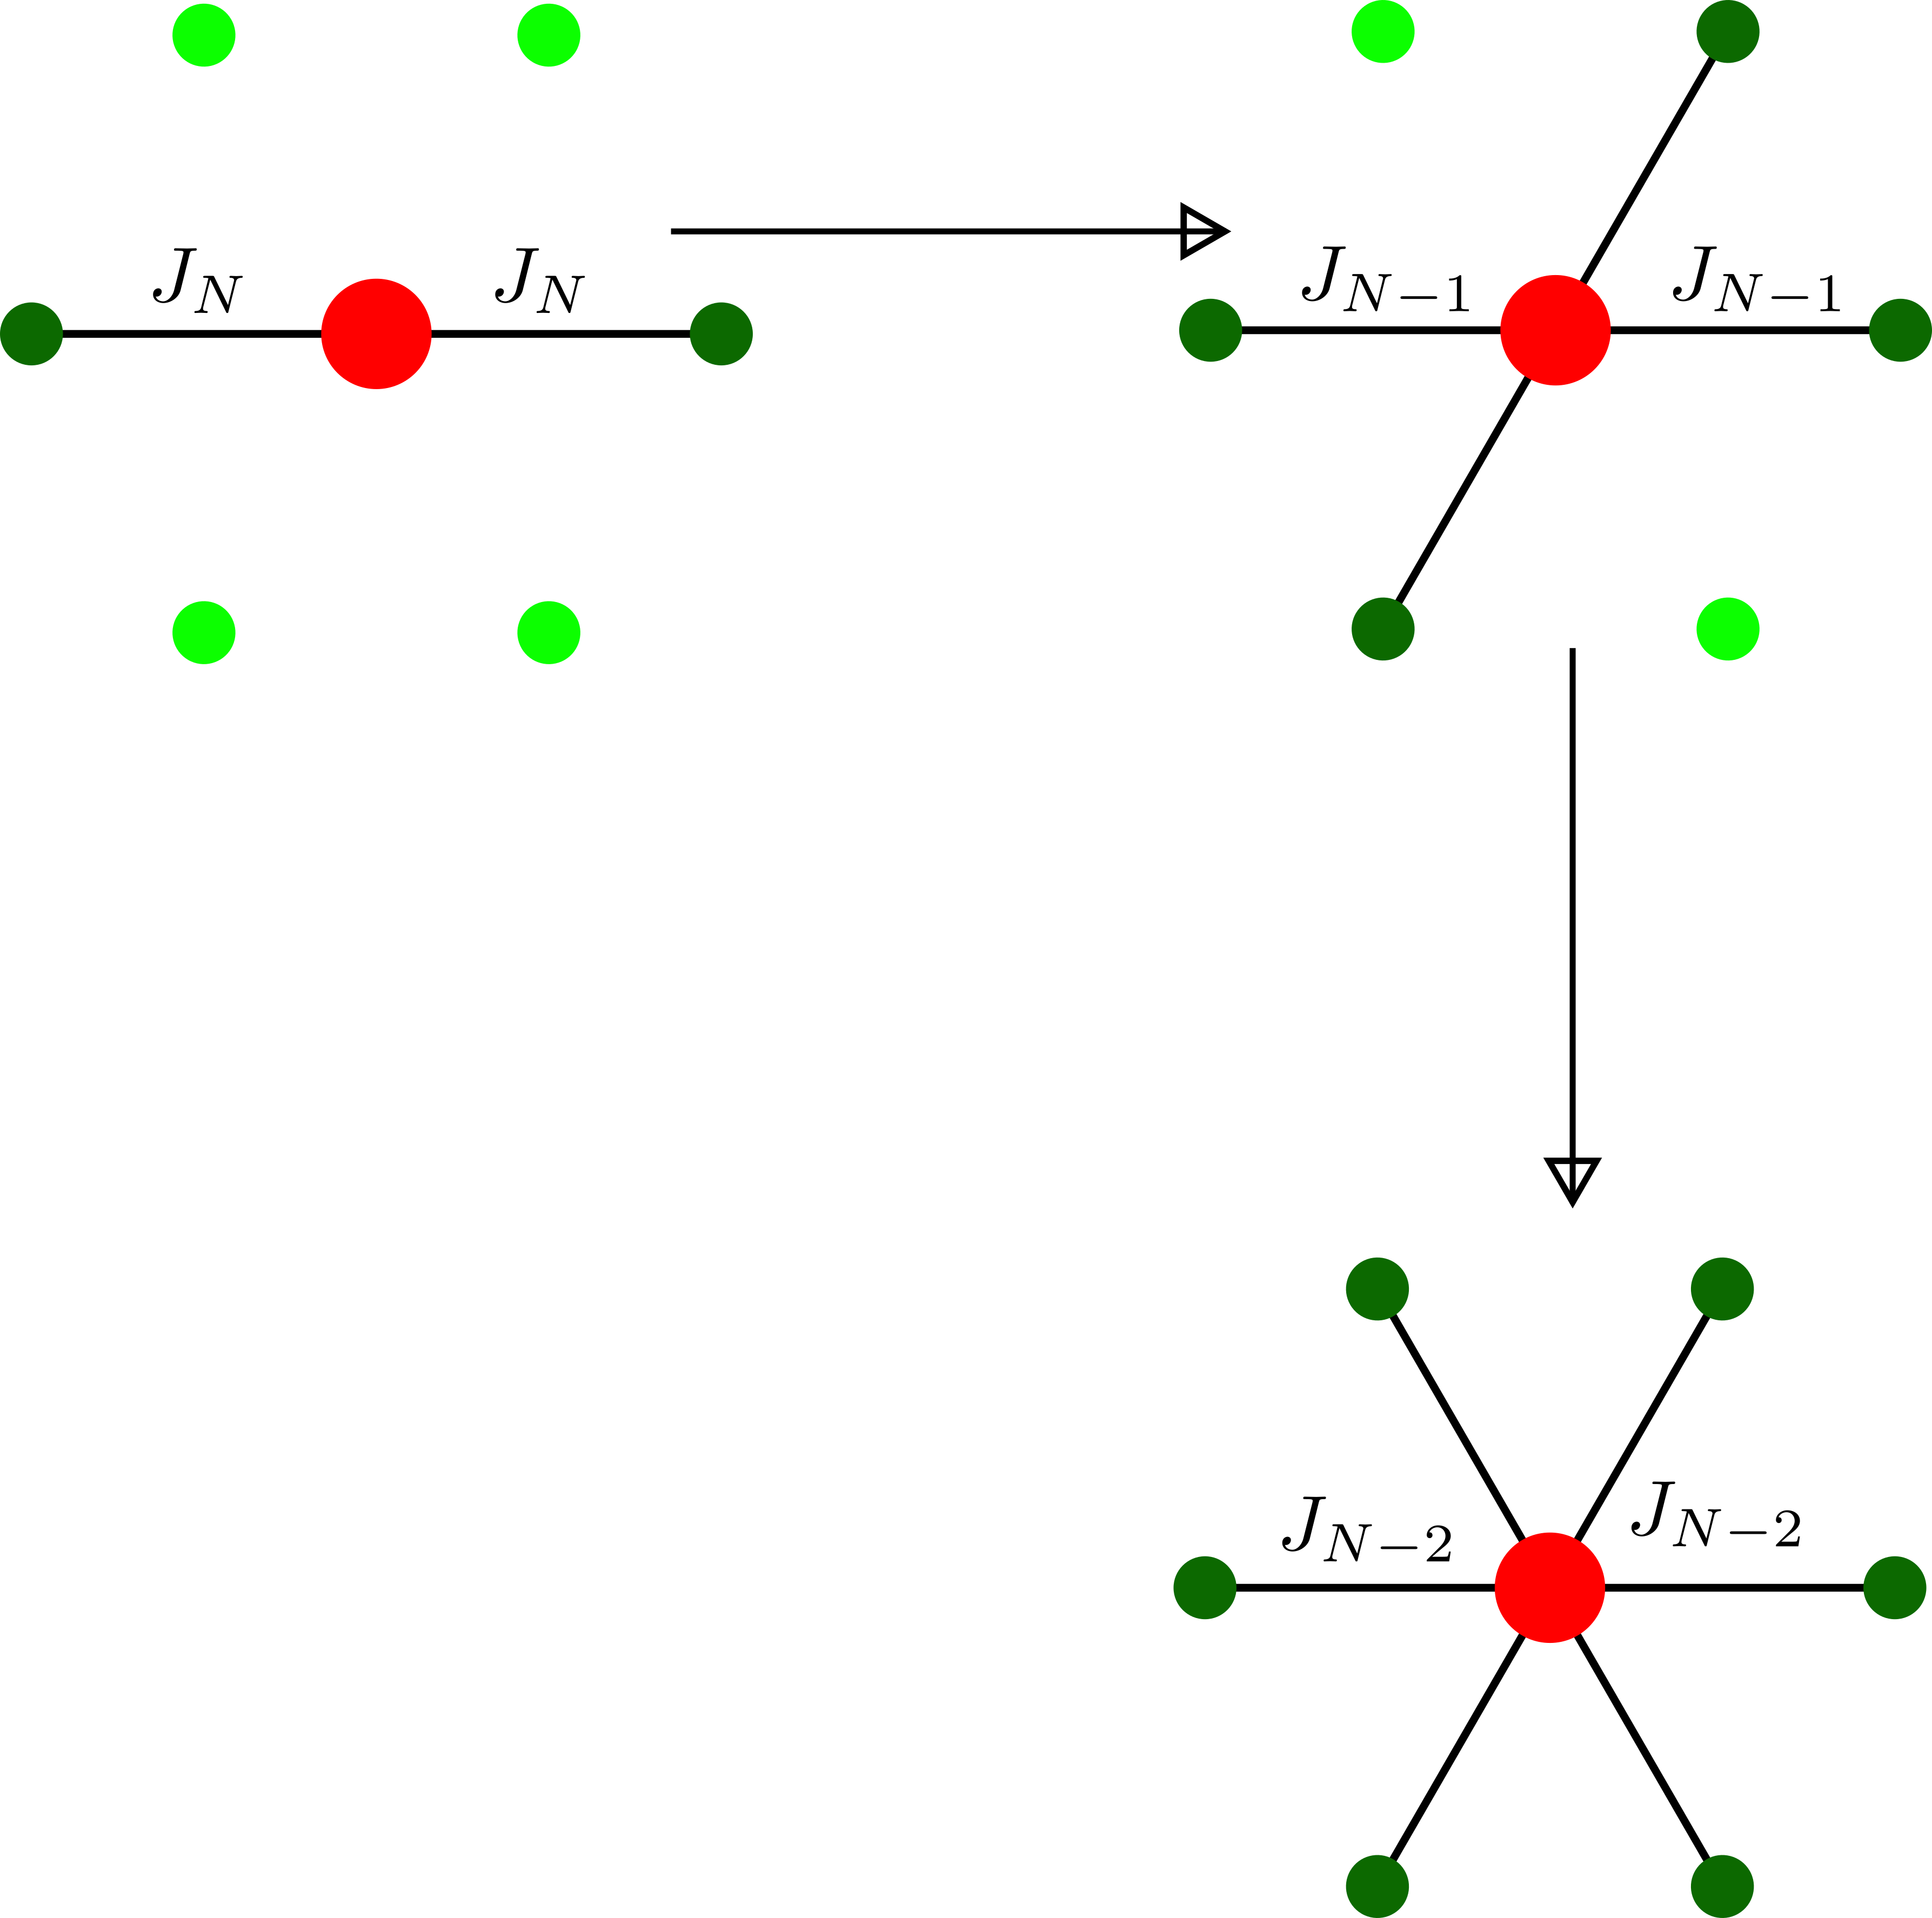
\includegraphics[width=0.45\textwidth]{figures/rev-rg-bonds-diag.png}
	\end{figure}
	\vspace*{\fill}
\footcite{am_thesis}
\end{frame}

\begin{frame}[noframenumbering]{Results: Reverse RG: Mutual Information}
	\hspace*{\fill}	\(I(A:B) = S_A + S_B - S_{AB}\)\hspace*{\fill}\(S_A = -\text{Tr }\left[\rho_A \ln \rho_A\right]\)\hspace*{\fill}
	\begin{figure}[htpb]
		\centering
		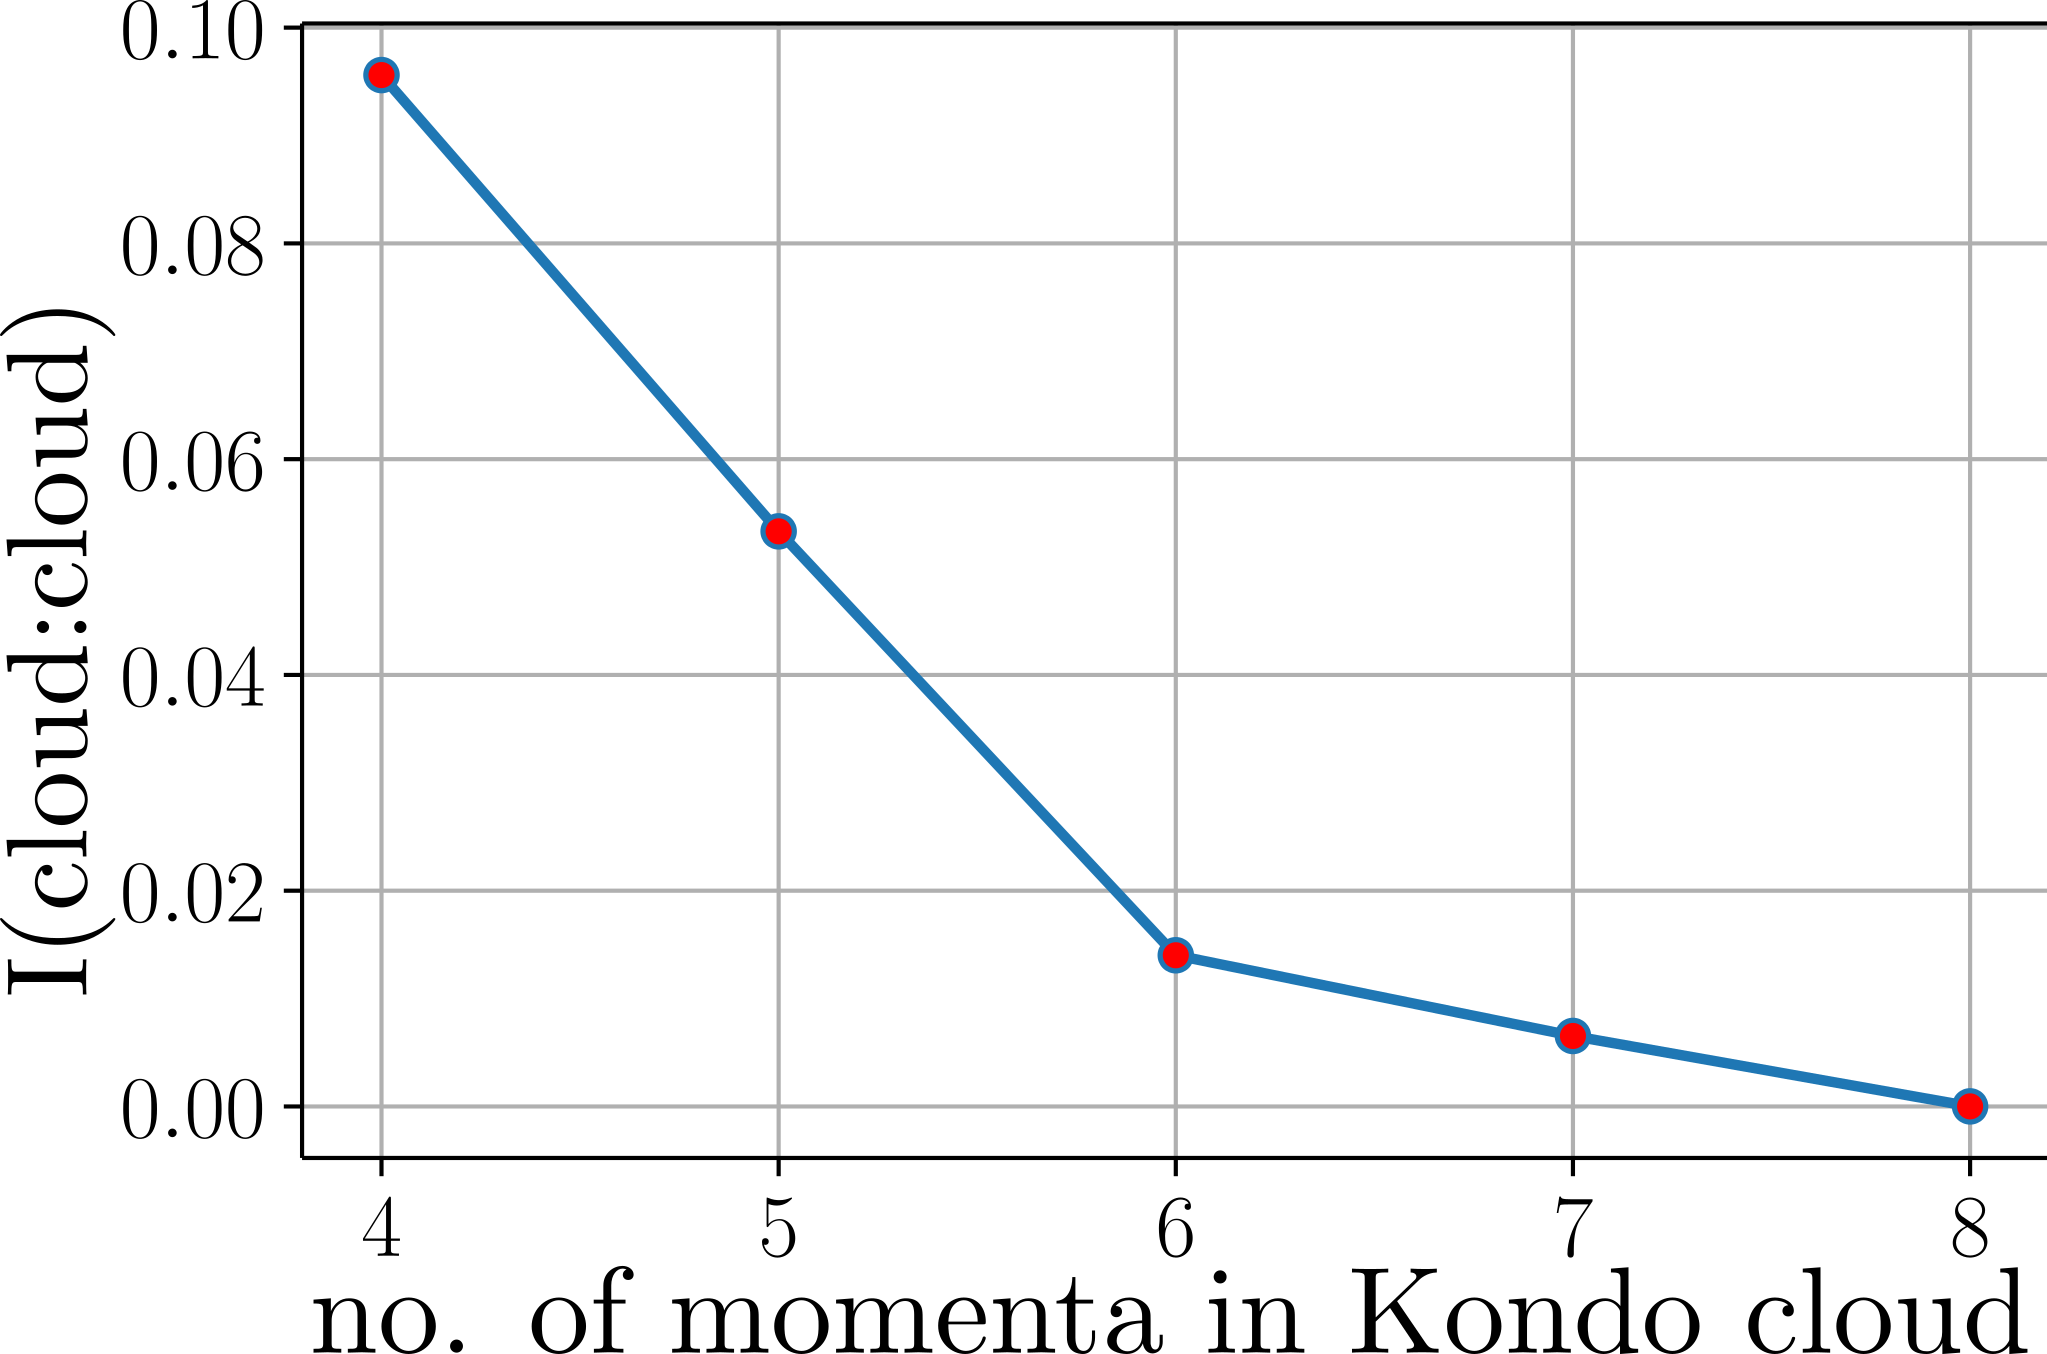
\includegraphics[width=0.45\textwidth]{figures/mutI_ee.png}\hspace*{\fill}
		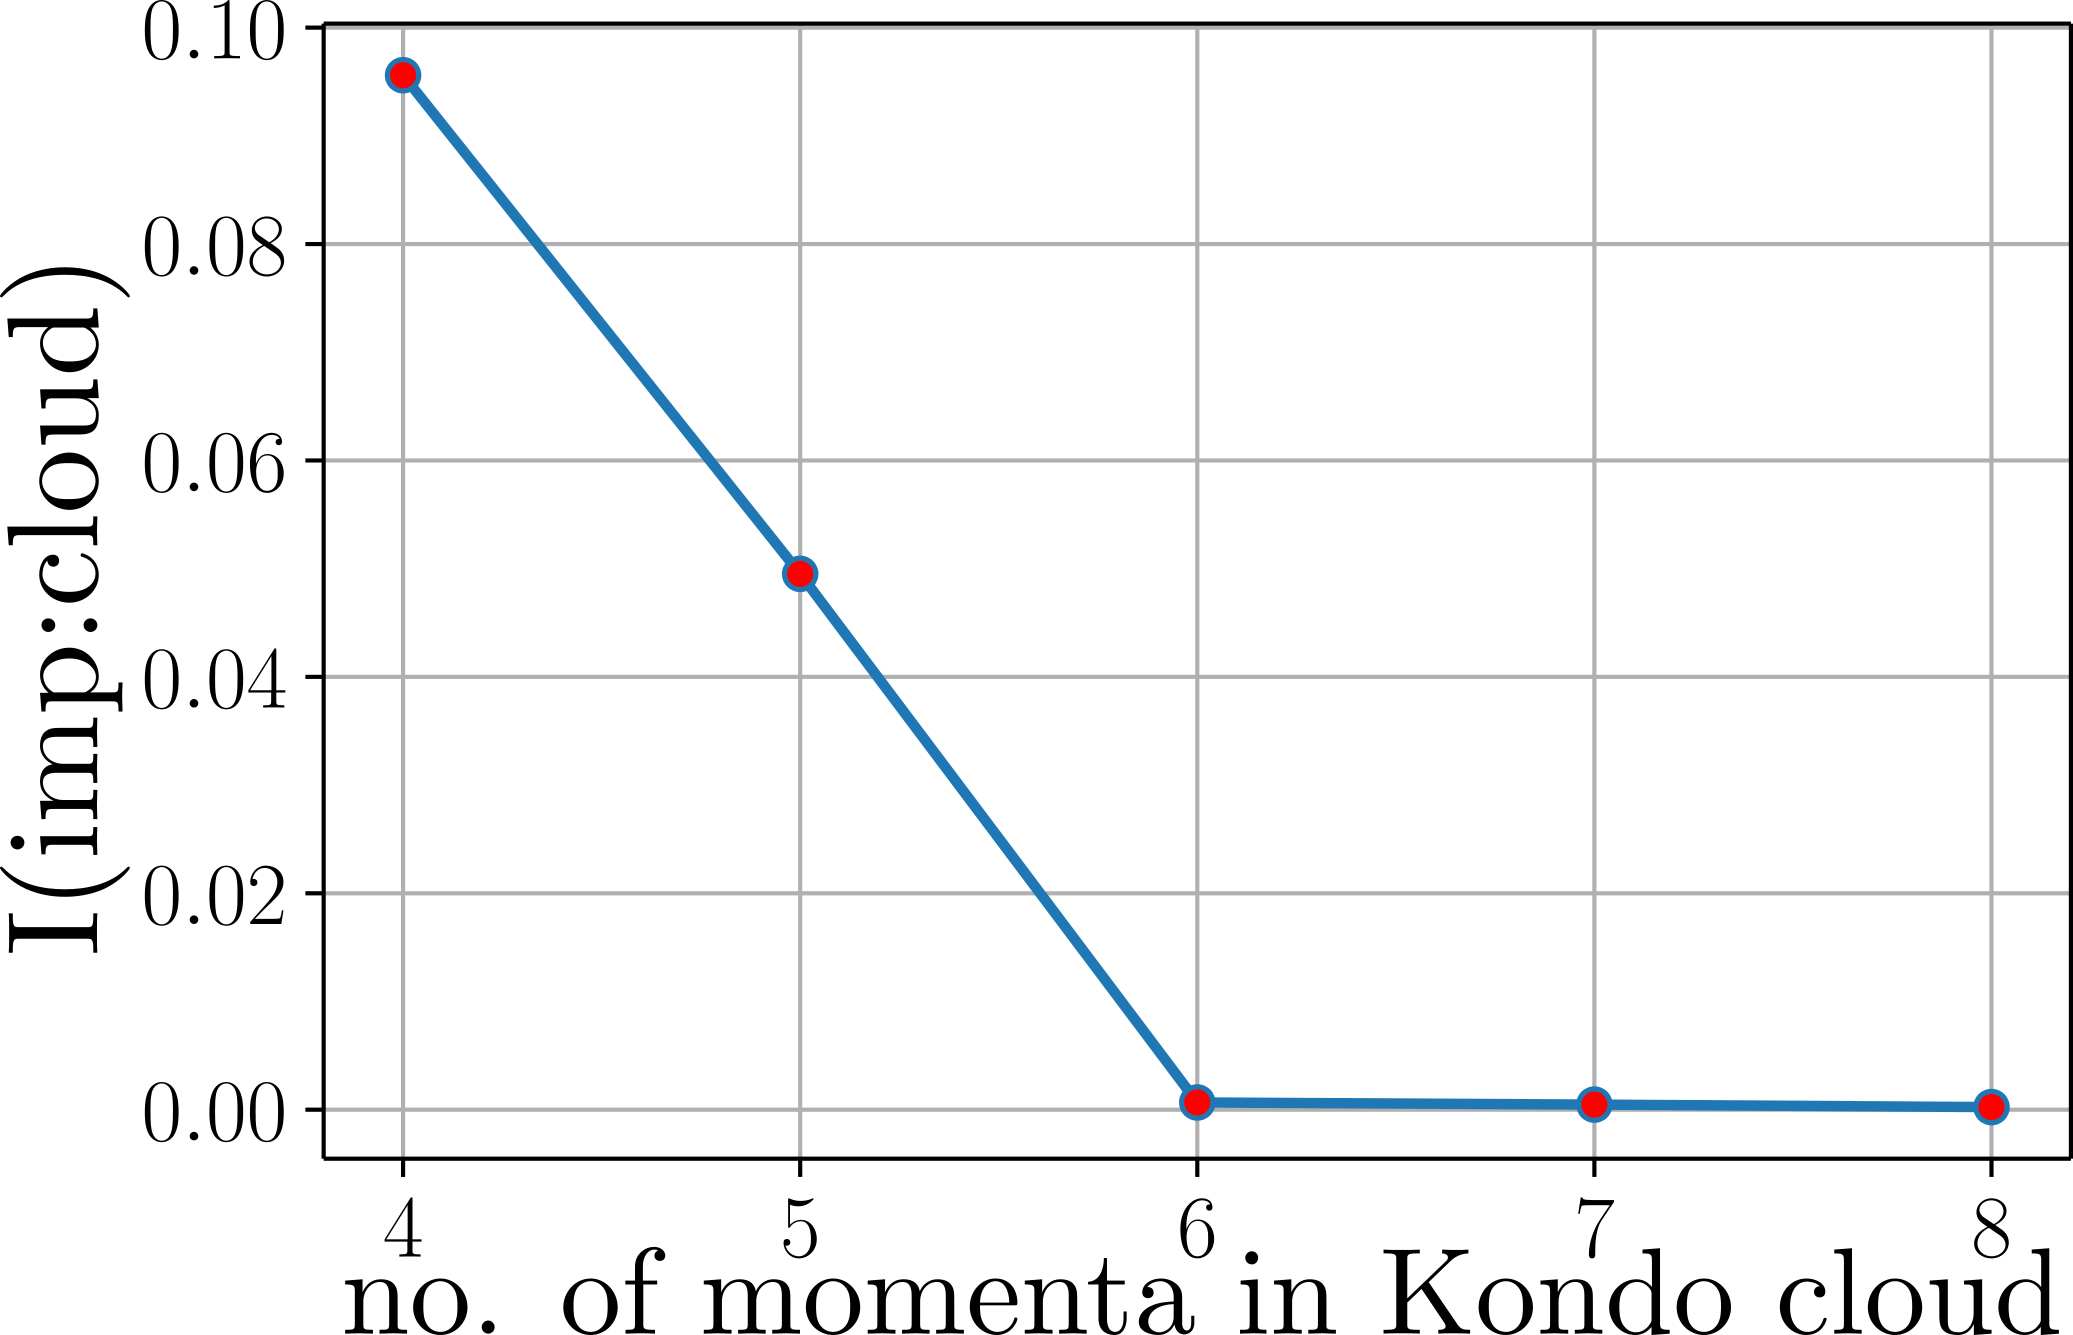
\includegraphics[width=0.45\textwidth]{figures/mutI_ed.png}
	\end{figure}
\end{frame}


\begin{frame}[noframenumbering]{Results: Reverse RG: Correlations}
	\begin{figure}[htpb]
		\centering
		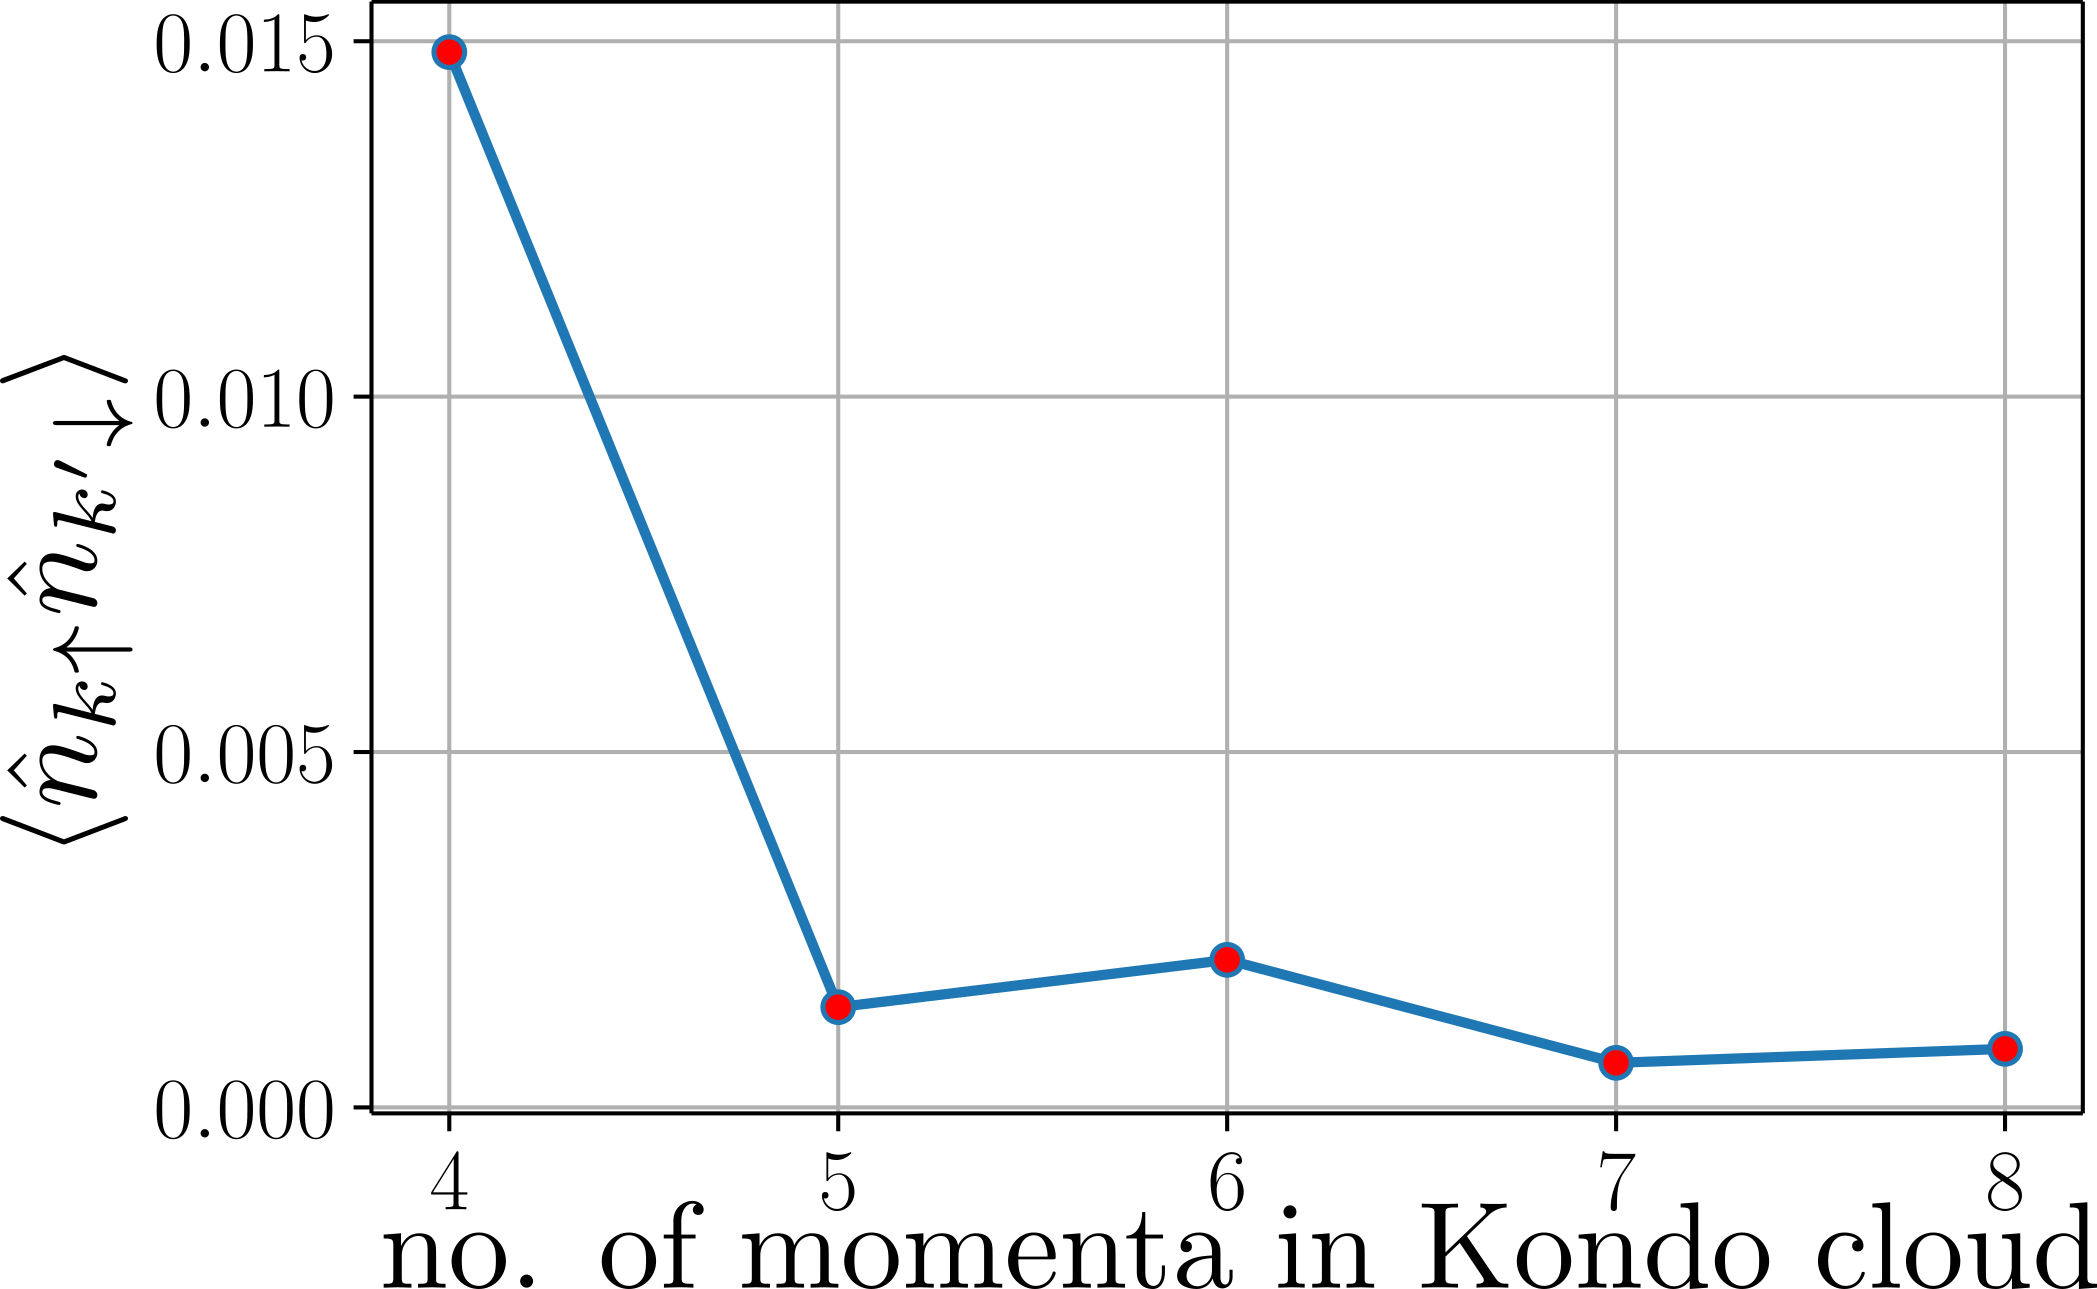
\includegraphics[width=0.45\textwidth]{figures/corr_diag.png}\hspace*{\fill}
		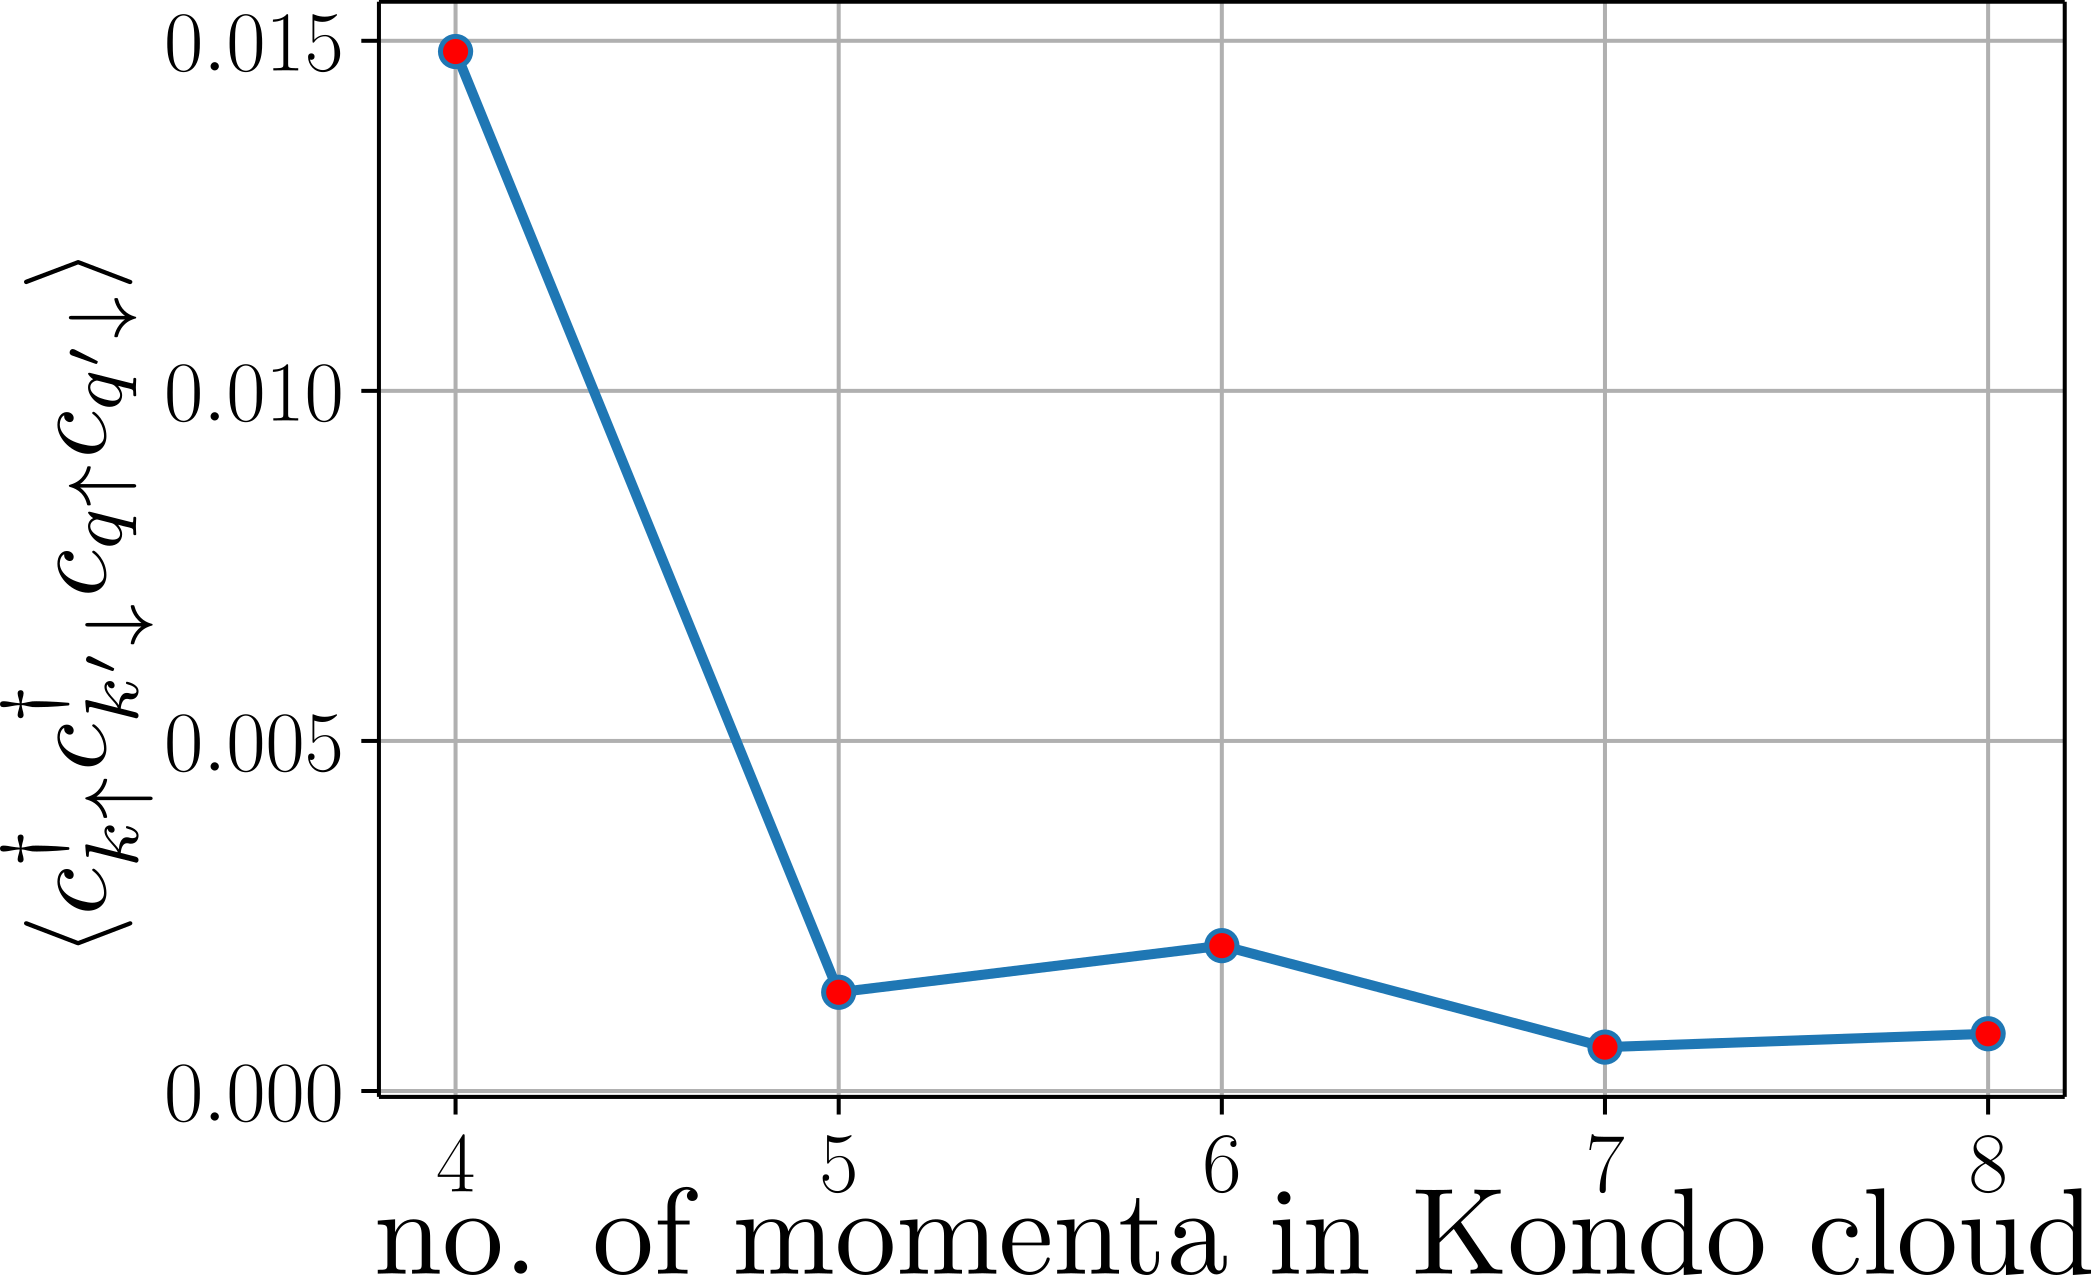
\includegraphics[width=0.45\textwidth]{figures/corr_od.png}
	\end{figure}
\end{frame}

\begin{frame}[noframenumbering]{Results: Luttinger's Theorem}
	\hspace*{\fill}	{\Large \(\overbrace{N}^{\text{total no. of}\atop{\text{ particles}}} = \overbrace{P_{\text{Det }G_d}(\Gamma_<) + \frac{1}{2}P_{\text{Det }G_d}(\Gamma_0)}^{\text{no. of poles of}\atop{\text{imp. Greens func.}}} + \overbrace{V_L}^{\text{no. of poles of}\atop{\text{cbath Greens func}}}\)}\hspace*{\fill}
\begin{equation*}\begin{aligned}
	P_X(C) &\equiv \frac{1}{2\pi i}\oint_C dz \frac{\partial{\ln X}}{\partial{z}} &&=\text{no. of poles of } X \text{ enclosed by curve }C \\
	       &= \frac{1}{2\pi i}\oint_{C(X)} \frac{dX}{X} &&= \text{winding number of } X \text{ around }X(C)
\end{aligned}\end{equation*}
\begin{minipage}{0.4\textwidth}
	\begin{figure}[htpb]
		\centering
		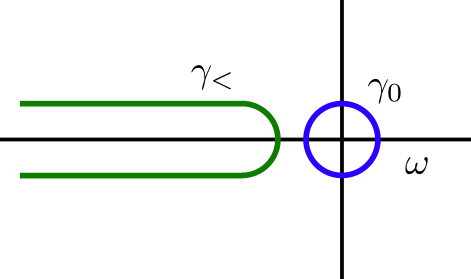
\includegraphics[width=0.9\textwidth]{figures/contours.png}
	\end{figure}
\end{minipage}
\hspace*{0.15\textwidth}
\begin{minipage}{0.4\textwidth}
	\begin{figure}[htpb]
		\centering
		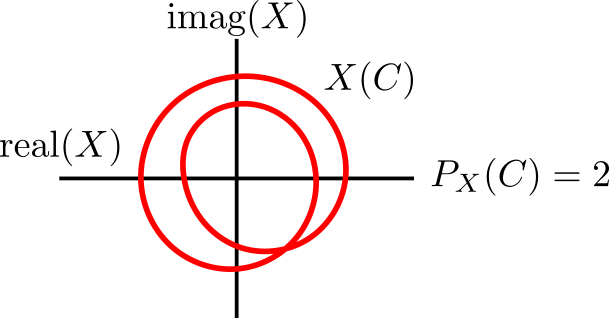
\includegraphics[width=0.9\textwidth]{figures/wind_num.png}
	\end{figure}
\end{minipage}
\footcite{seki}
\end{frame}

\begin{frame}[noframenumbering]{Results: Luttinger's Theorem}
\begin{minipage}{0.6\textwidth}
\begin{figure}[htpb]
	\centering
	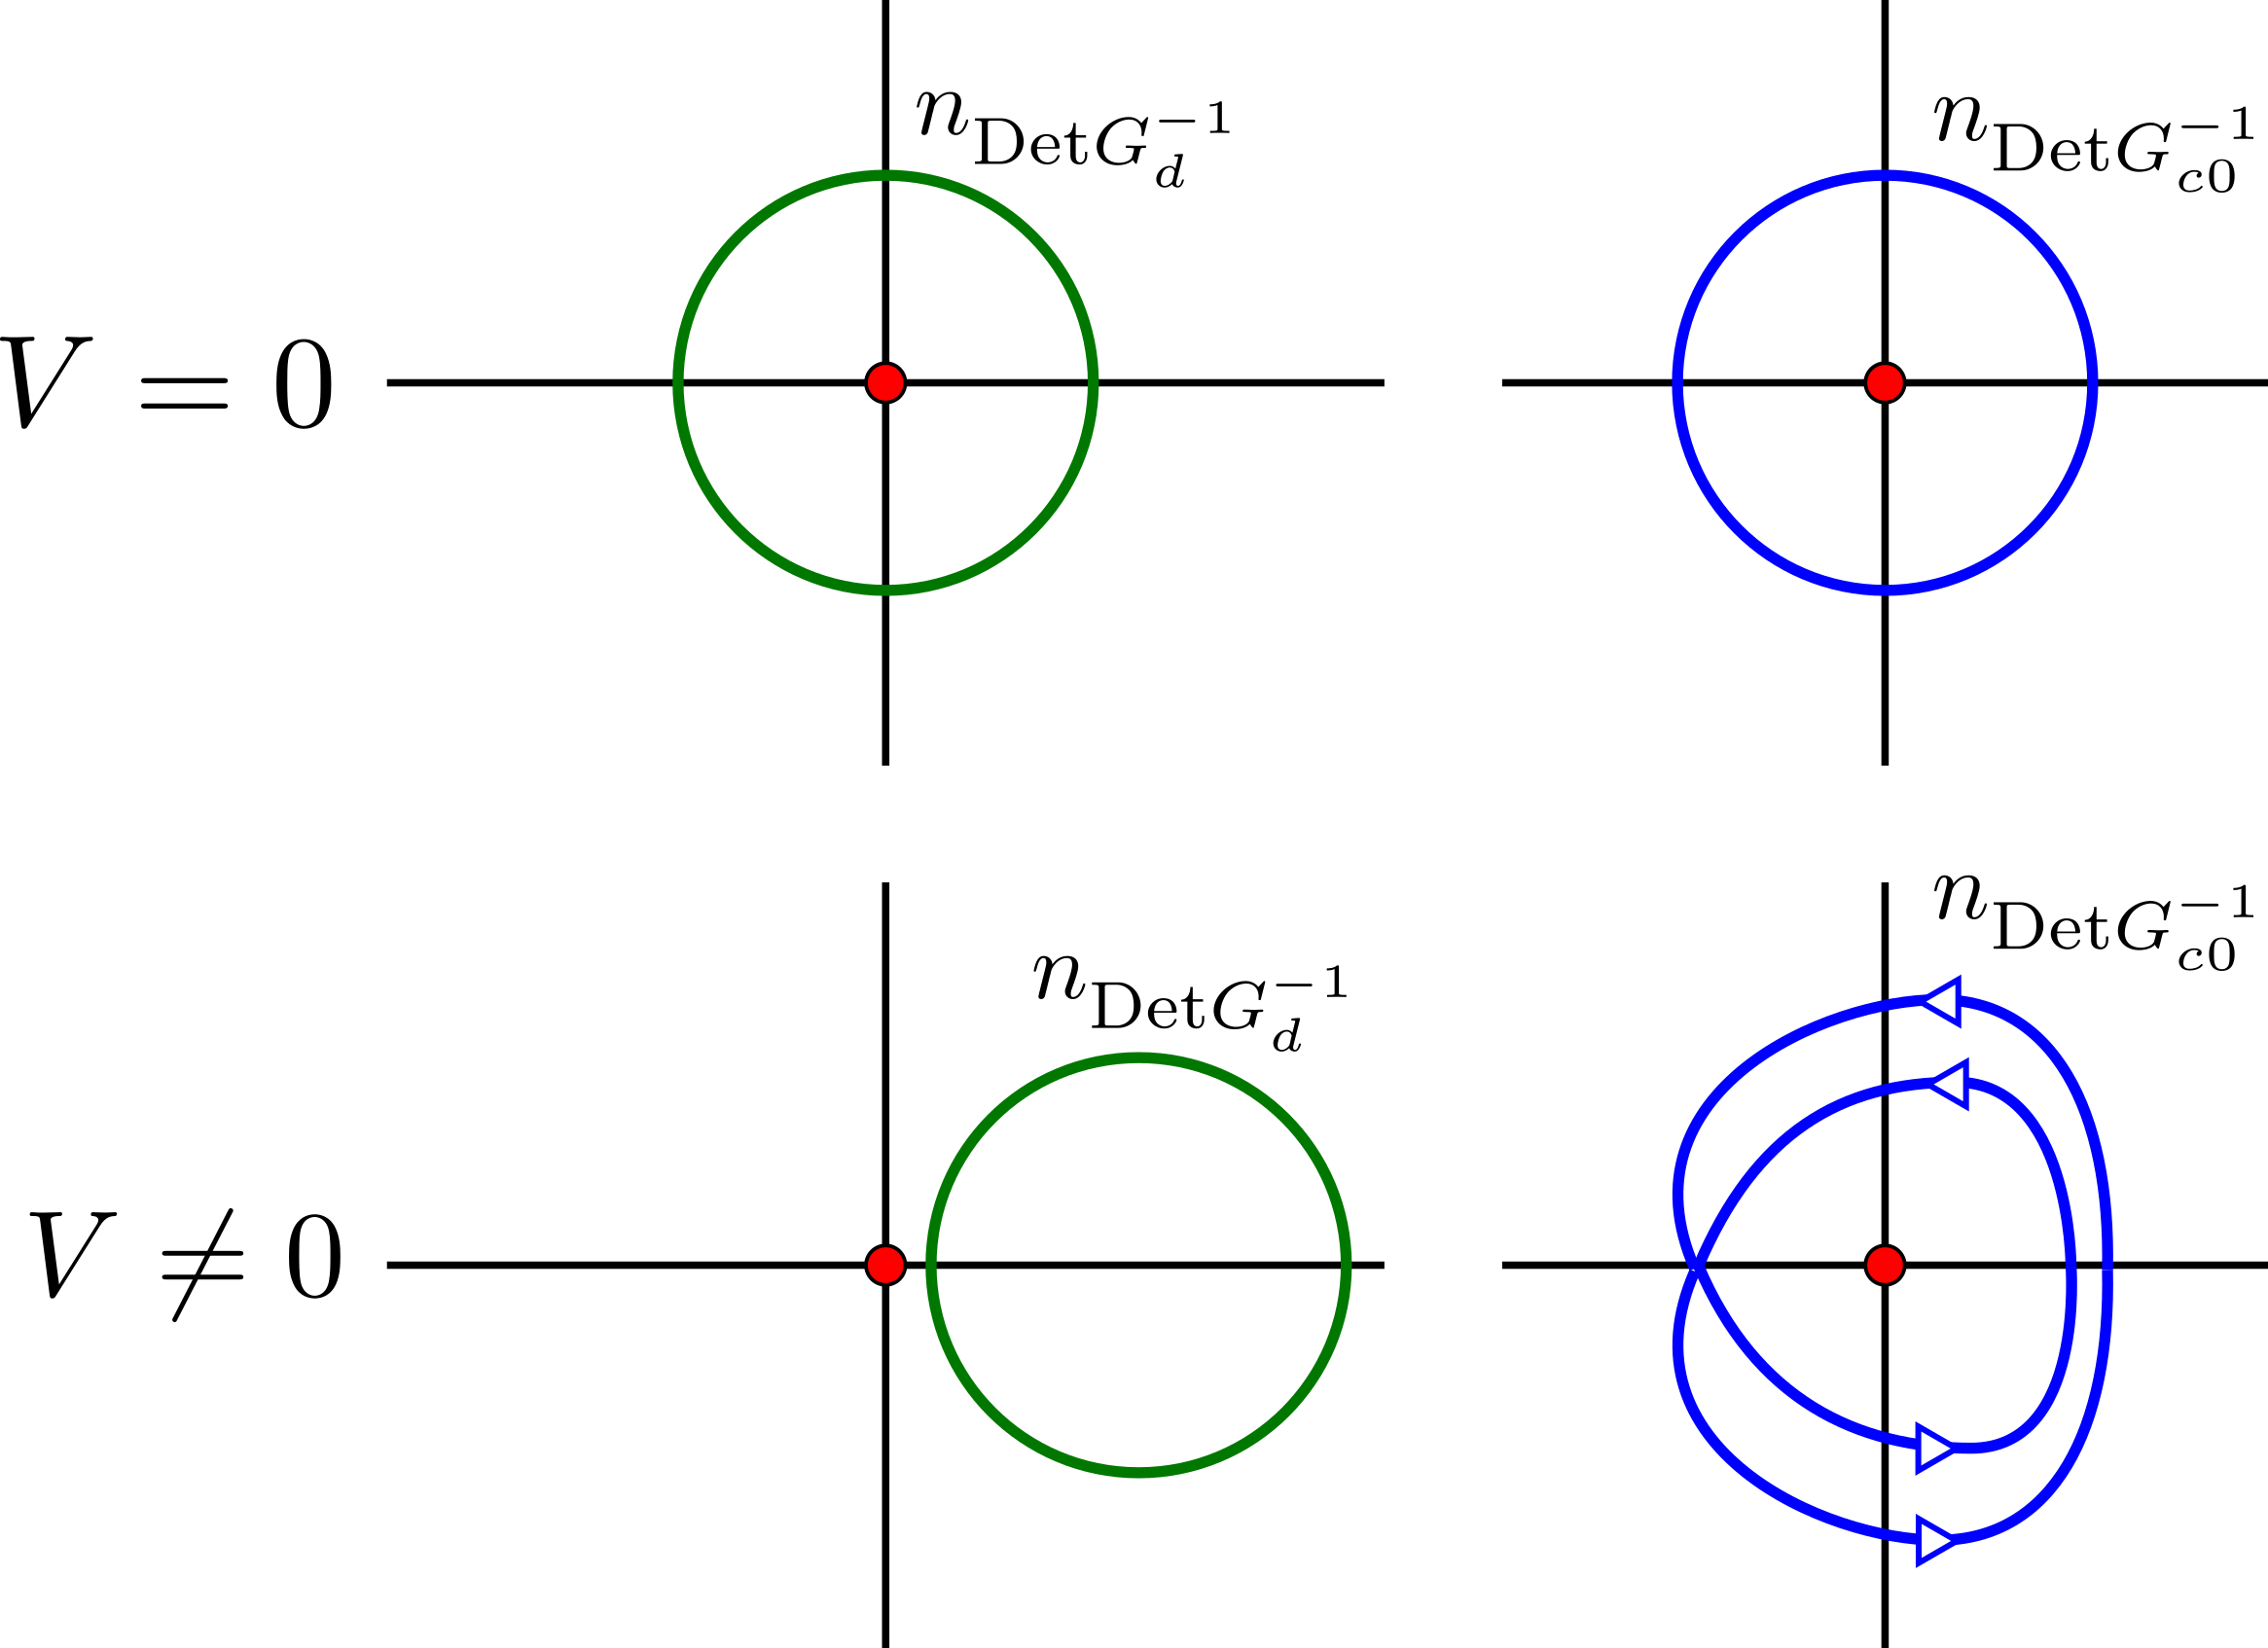
\includegraphics[width=0.75\textwidth]{figures/luttinger_top_change.png}
\end{figure}
\end{minipage}
\begin{minipage}{0.39\textwidth}
	\vspace*{5pt}
	{\large \[n_{\text{Det }G_d^{-1}} = 1\]
	\vspace*{45pt}
	\[n_{\text{Det }G_d^{-1}} = 0\]}
\end{minipage}
\vspace*{10pt}
\cen{
	\Large
	\(V_L = V_L^0 + 1\)
}
\footcite{martin}
\end{frame}

\begin{frame}[noframenumbering]{Results: Local Fermi Liquid}
	\[H^* = \overbrace{J^* \vec{S_d}\cdot\vec{s} + K^* \vec{C_d}\cdot\vec{c} + V^* \left( c^\dagger_{d\sigma}c_{0\sigma} + \text{h.c.} \right)}^\text{solve exactly} + \overbrace{t\sum_{\left<i,j \right>}c^\dagger_{i\sigma}c_{j\sigma}}^\text{treat as perturbation}\]
	\hspace*{0.5\textwidth}$\Bigg\downarrow$ \(4^\text{th}\) fourth order pert.
	\[E_1^{(4)} = -\frac{16t^4}{3{J^*}^3}, E_2^{(4)} = -\frac{16t^4}{9{J^*}^3}\]
	\[H^* \sim J^* \vec{S_d}\cdot\vec{s} + K^* \vec{C_d}\cdot\vec{c} + V^* \left( c^\dagger_{d\sigma}c_{0\sigma} + \text{h.c.} \right) + \overbrace{\frac{t^4}{{J^*}^3} \hat n_{1 \uparrow}\hat n_{1 \downarrow}}^\text{local Fermi liquid}\]

\vspace*{-10pt}
\footcite{nozieres}
\end{frame}

\begin{frame}[noframenumbering]{Results: Wilson Ratio (\(T=0\))}
\vspace*{-10pt}
\cen{
	\text{thermal average:} \(\left<\hat n_{1 \uparrow}\hat n_{1 \downarrow}\right> \xrightarrow{\text{mean field}\atop \text{approximation}} \left<\hat n_{1 \uparrow}\right>\left<\hat n_{1 \downarrow}\right>\)\\[20pt]
\scalebox{1.5}{
	\(\epsilon_{k\sigma} = \epsilon_k^0 + \sum_q f_{kq}\left<n_{q\overline\sigma} \right>\)
}
}
\vspace*{\fill}
\hspace*{60pt}
\begin{minipage}{0.25\textwidth}
\begin{itemize}
	\item \(f_{\uparrow\uparrow} =0\)
	\item \(\chi_c(T\to 0) =0\)
\end{itemize}
\end{minipage}
\begin{minipage}{0.15\textwidth}
	\scalebox{2}{$\longrightarrow$}
\end{minipage}
\begin{minipage}{0.33\textwidth}
\begin{itemize}
	\item \(C_v(T\to 0) = \rho_\text{imp}T\)
	\item \(\chi_s(T \to 0) = 2\rho_\text{imp}\)
\end{itemize}
\end{minipage}
\hspace*{20pt}
\vspace*{\fill}
\cen{
	\scalebox{1.5}{
	$R = \frac{\chi_s}{\frac{C_v}{T}} = 2$
}
}

\footcite{hewsonp}
\end{frame}

\begin{frame}[noframenumbering]{Results: Relation between \(R\) and \(\Delta V_L\)}
	\begin{minipage}{0.43\textwidth}
		\begin{itemize}
			\item particle-hole symmetry
			\item strong-coupling fixed-point
			\item \(T=0\)
		\end{itemize}
	\end{minipage}
	\begin{minipage}{0.18\textwidth}
		\cen{
			\LARGE\(\longrightarrow\)
	}
	\end{minipage}
	\begin{minipage}{0.22\textwidth}
		\Large\(R = 1 + \sin^2 \delta(0)\)
	\end{minipage}
	\\[30pt]
	\begin{minipage}{0.43\textwidth}
		\begin{itemize}
			\item Friedel's sum rule 
			\item scattering theory arguments
		\end{itemize}
	\end{minipage}
	\begin{minipage}{0.18\textwidth}
		\cen{
			\LARGE\(\longrightarrow\)
	}
	\end{minipage}
	\begin{minipage}{0.25\textwidth}
		\Large\(\frac{1}{\pi}\delta(0) = \tilde N = \Delta V_L\)
	\end{minipage}
	\\[30pt]

	\cen{
		\Large\(R = 1 + \sin^2 \left( \pi \Delta V_L \right) \)\\[10pt]
		\Large\(\Delta V_L = 1 \longrightarrow R = 2 \)
}

\end{frame}
% \only<1>{
% \begin{flalign*}
% 	\mathcal{H} = \overbrace{\sum_{k\sigma}\epsilon_k \hat n_{k\sigma} + \sum_{k\sigma}\left[V(k)c^\dagger_{k\sigma}c_{d\sigma} + \text{h.c.}\right] + \epsilon_d \sum_\sigma \hat n_{d\sigma} + U\hat n_{d\uparrow}\hat n_{d\downarrow}}^{SIAM}\\
%  + \underbrace{J \vec{S_d}\cdot \sum_{kq\alpha\beta}\vec{\sigma}_{\alpha,\beta}c^\dagger_{k\alpha}c_{q\beta}}_\text{spin-exchange}+ \underbrace{J \vec{C_d}\cdot \sum_{kq\alpha\beta}\vec{\sigma}_{\alpha,\beta}\psi^\dagger_{k\alpha}\psi_{q\beta}}_\text{isospin-exchange}
% \end{flalign*}
% }
% \only<2-3>{\Large{\textbf{RG Equations}}
% \only<2>{
% 	\vspace*{-15pt}
% 		\begin{equation*}\begin{aligned}\Delta U &= \left(U + \frac{1}{2}J\right)\sum_{|q|=\Lambda_n} \frac{|V(q)|^2}{(\omega - \epsilon_q - \frac{1}{2}U - \frac{1}{4}J)(\omega - \epsilon_q)}\\[5pt]
% 			\Delta V(q) &= -\frac{3}{4}J\sum_{|q|=\Lambda_n} \frac{V(q)}{\omega - \epsilon_q - \frac{1}{2}U - \frac{1}{4}J}\\[5pt]
% \Delta J &= -\frac{1}{4}J^2\sum_{|q|=\Lambda_n\atop{k<\Lambda_n}} \frac{1}{\omega - \epsilon_q - \frac{1}{2}U - \frac{1}{4}J}\end{aligned}\end{equation*}
% }
% \only<3>{
% 	\vspace*{25pt}
% \begin{itemize}
% 	\item Particle-hole symmetric
% 	\vspace*{10pt}
% 	\item Hermitian
% 	\vspace*{10pt}
% 	\item \(SU(2)\)-symmetric
% 	\vspace*{10pt}
% 	\item Reduce to Poor Man's scaling and Kondo 1-loop forms
% \end{itemize}
% }
% }
% \end{frame}

% \begin{frame}[noframenumbering]{Results (\(\pmb{J=0}\))}
% \vspace*{-10pt}
% \begin{figure}
% \def\svgwidth{\columnwidth}
% \centering
% \scalebox{1}{\input{lmflow.pdf_tex}}
% \end{figure}
% \only<1>{\vspace*{10pt}\centering 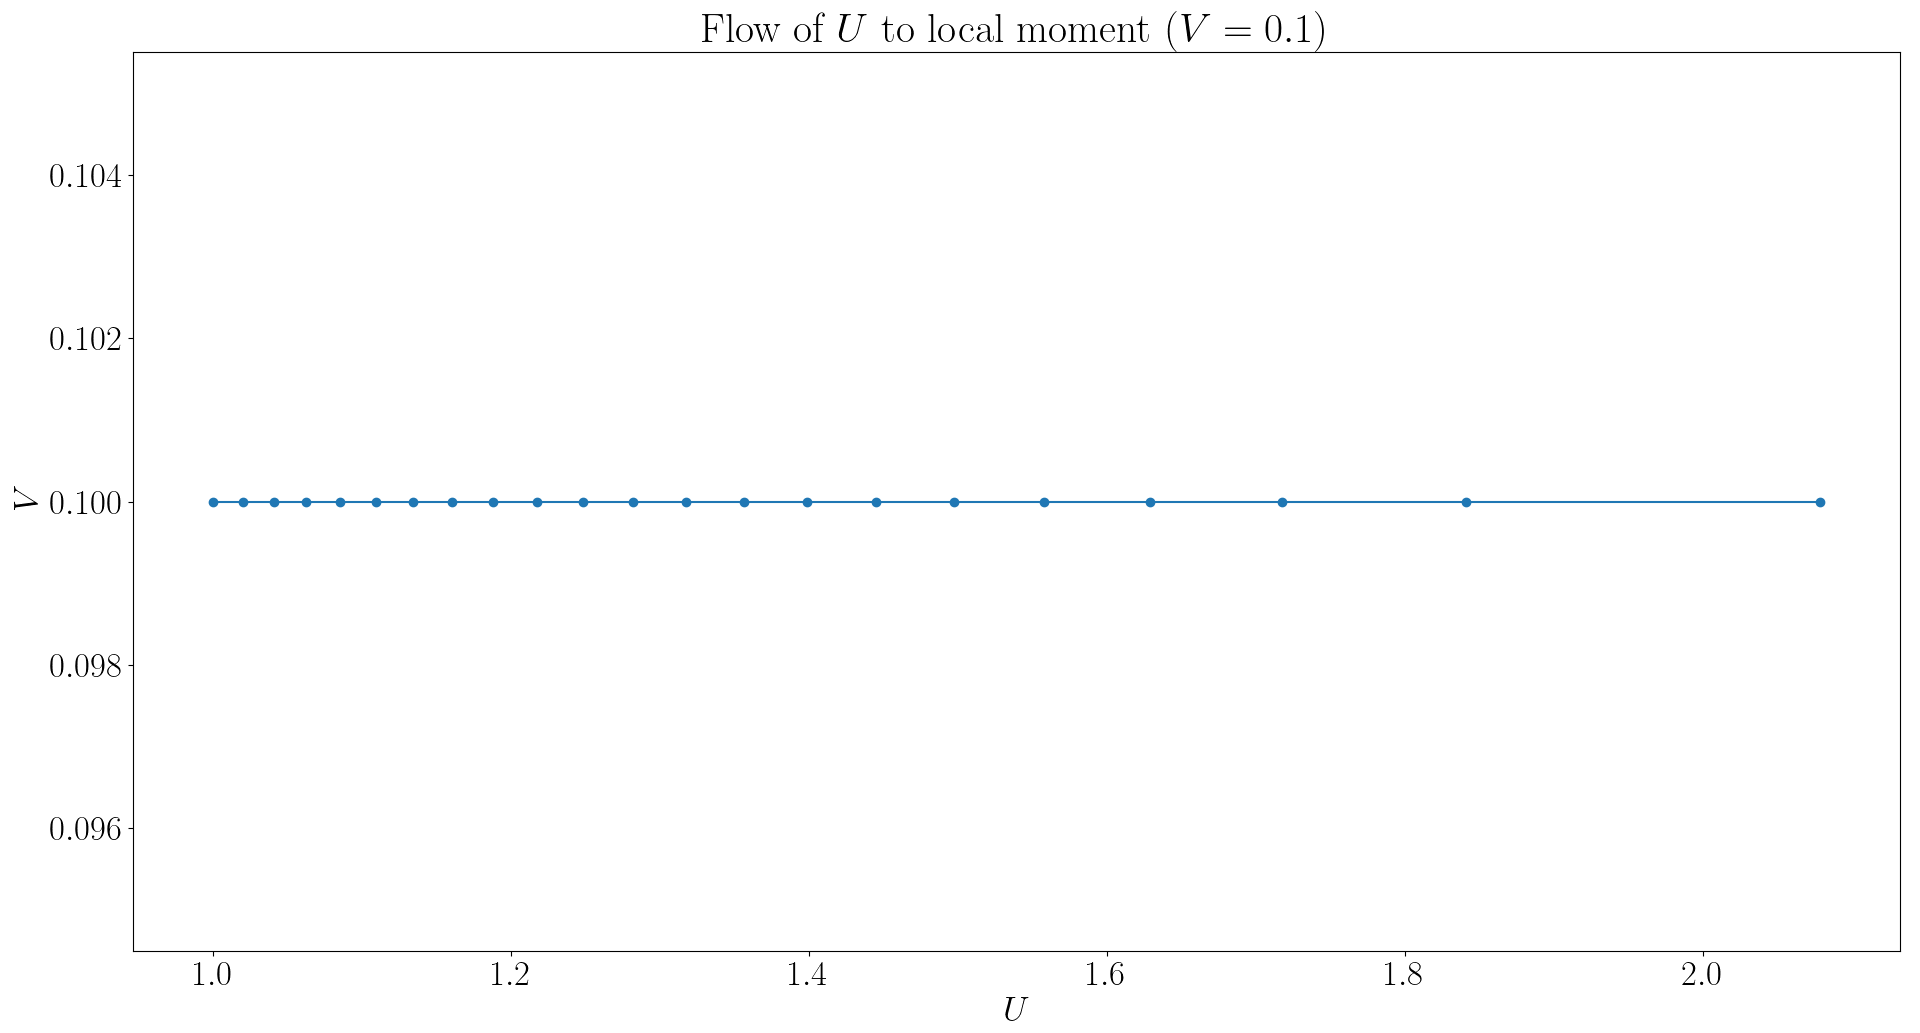
\includegraphics[scale=0.2]{fo2lm.png}}
% \begin{tabular}{cl}  
% \begin{tabular}{l}
% 	\hspace*{-30pt}\parbox{0.33\linewidth}{
% 		\vspace*{-10pt}
% 	\begin{itemize}\uncover<2->{\item \textbf{No separatrix} for the flows to the local moment} 
% 		\vspace*{10pt}
% 		\uncover<3>{\item Local moment forms at \textbf{finite \(U\)}.}
% \end{itemize}
%     }
%          \end{tabular}
%            &  \uncover<3>{ \begin{tabular}{c}
% 			   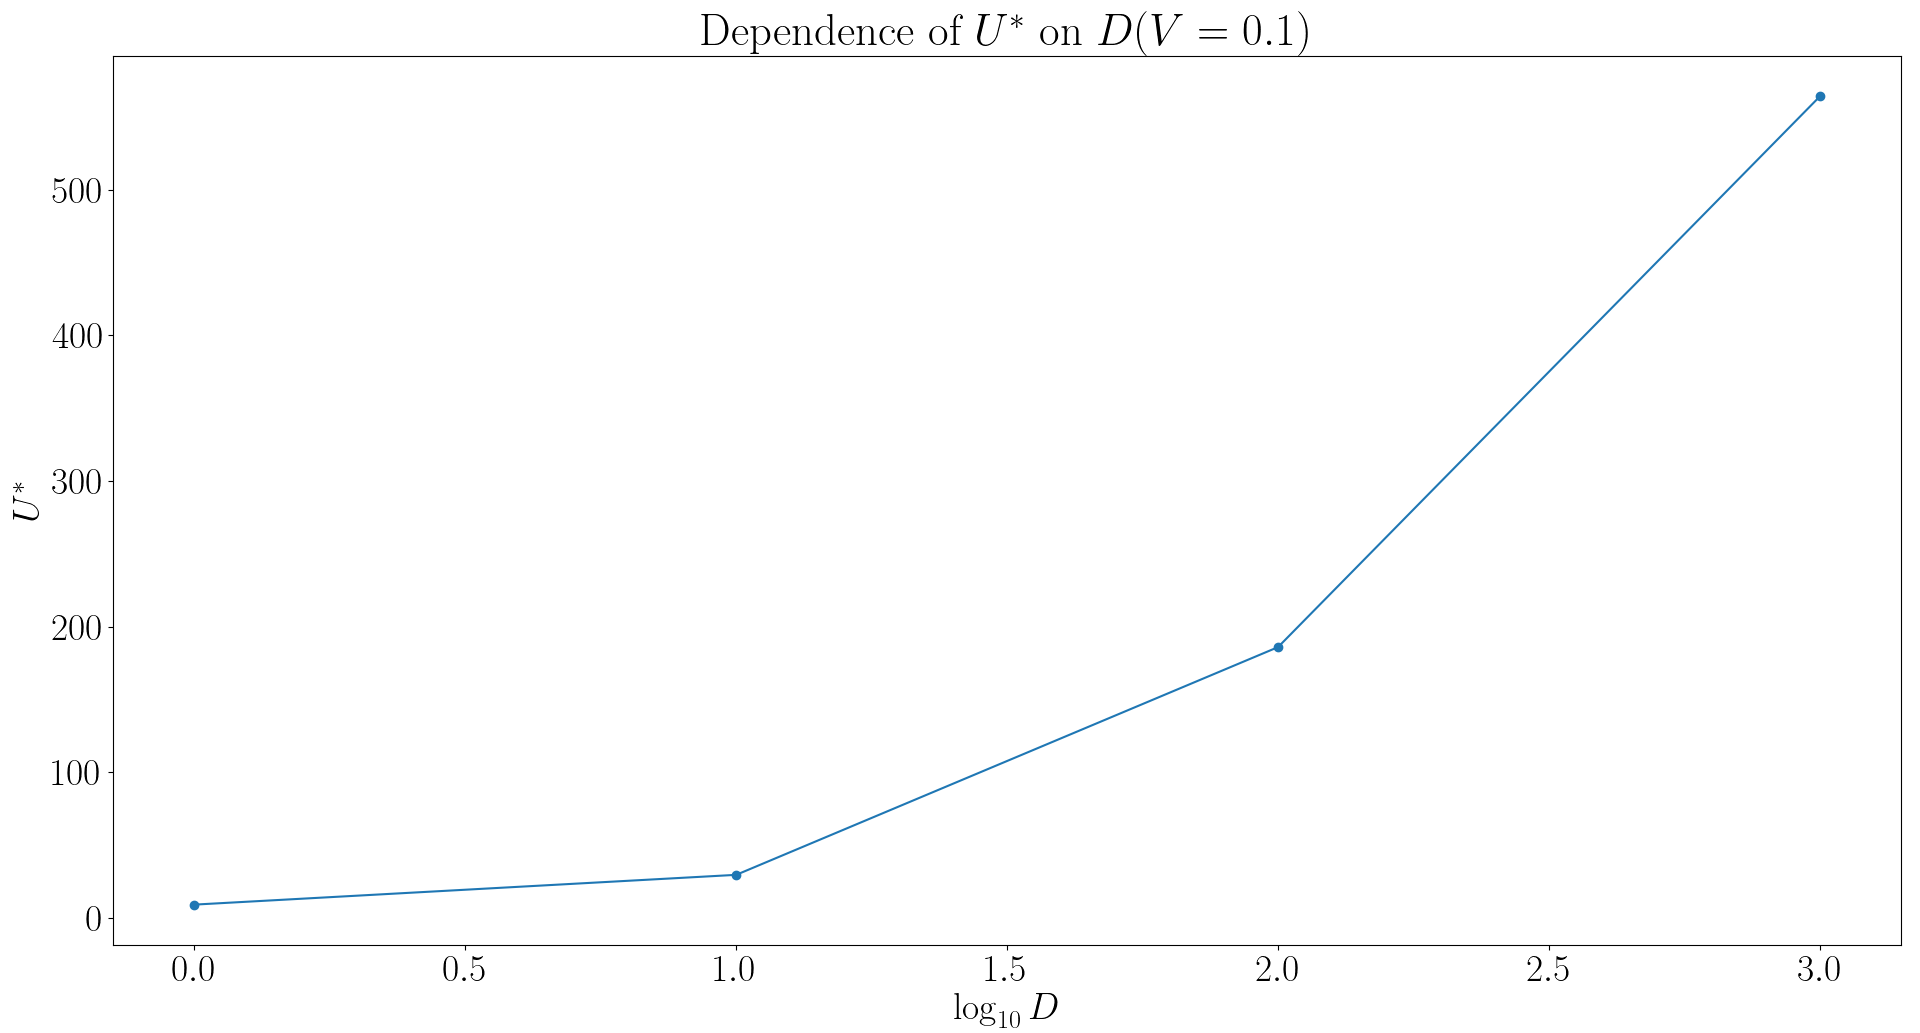
\includegraphics[scale=0.2]{UvsbareD.png}
% 	   \end{tabular}}\\
   
% \end{tabular}
% \end{frame}

% \begin{frame}[noframenumbering]{Results (\(\pmb{J>0}\))}
 
% \begin{tabular}{cl}  
% \begin{tabular}{l}
% \hspace*{-20pt}\parbox{0.5\linewidth}{
% \begin{itemize}
% \vspace*{-20pt}
% \item J now drives the flow towards strong-coupling fixed point.
% \vspace*{10pt}
% \item This is in contrast to the NRG flow diagram where \(\Delta \sim \frac{V^2}{U}\) was the driver of the flow.
% \end{itemize}
% }
% \end{tabular}
% & \begin{tabular}{c}
% \only<1>{    
% \centering 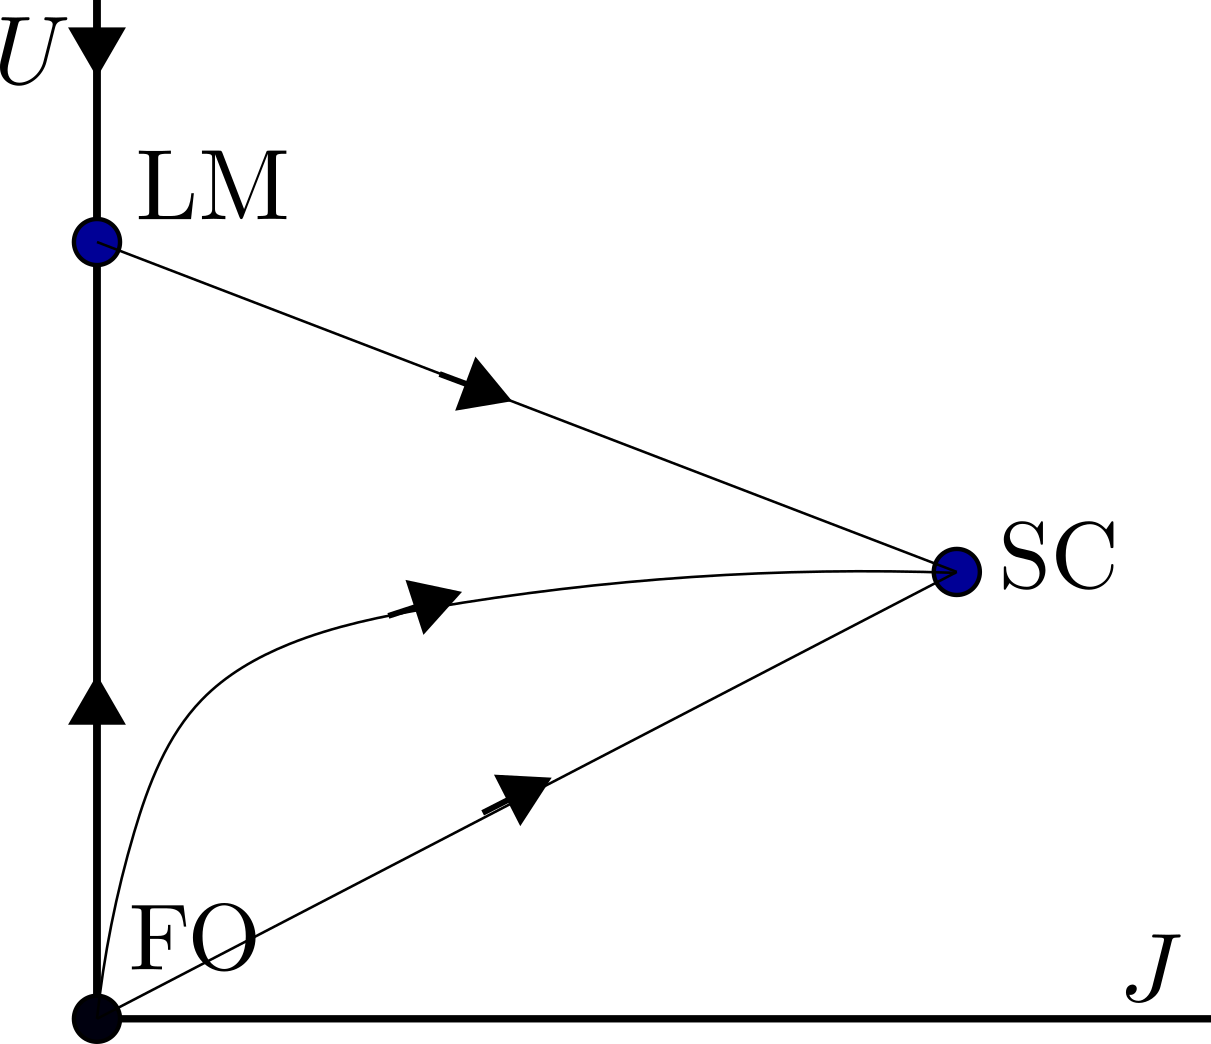
\includegraphics[scale=0.5]{schematic.png}
% }
% \only<2>{%
% 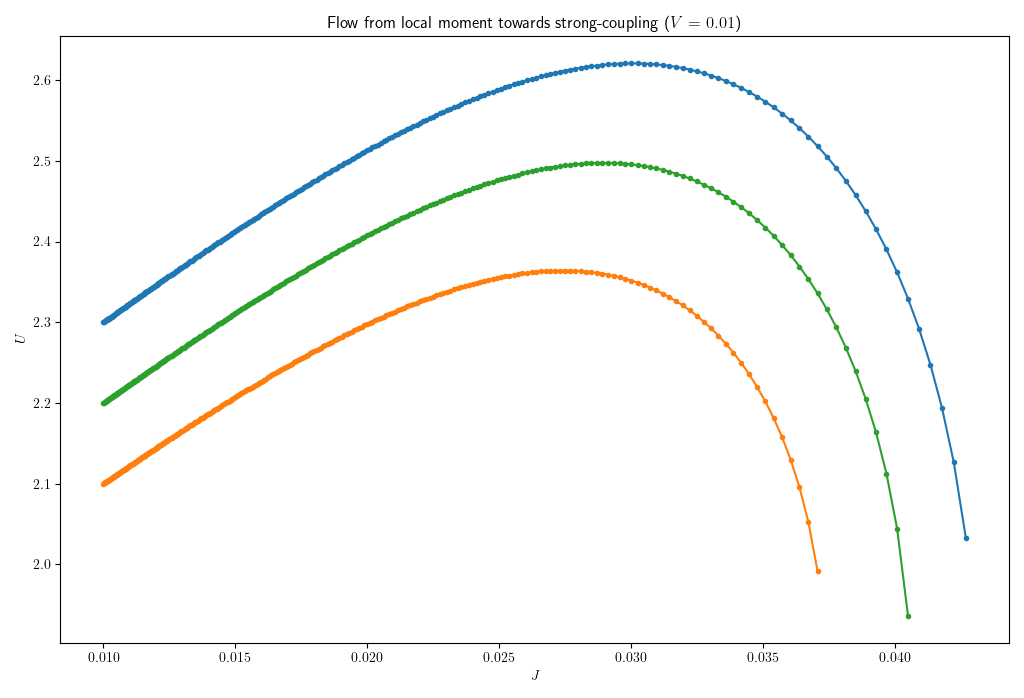
\includegraphics[width=0.35\textwidth]{lm2sc.png}\\
% \hspace*{5pt}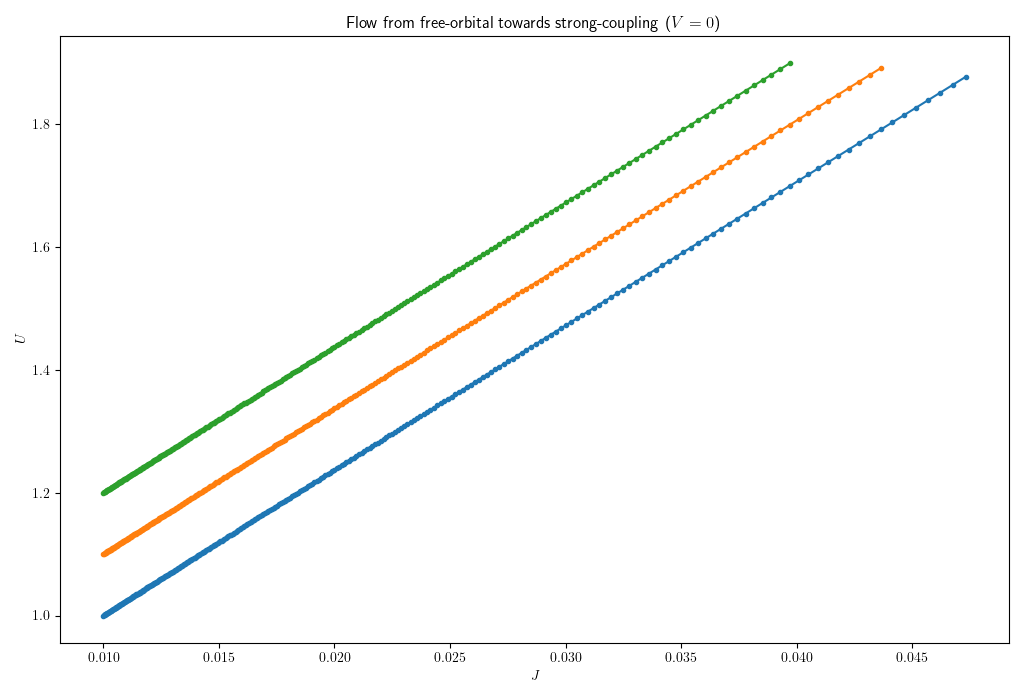
\includegraphics[width=0.35\textwidth]{fo2sc.png}
% }
% \end{tabular}
% \end{tabular}
\section{Summary of Results}
\begin{frame}[noframenumbering]{}
	\vspace*{-5pt}
	\begin{figure}[htpb]
		\centering
		
\includegraphics[width=\textwidth]{figures/summary.png}
	\end{figure}
\end{frame}

\section{Future Directions}
\begin{frame}[noframenumbering]{What's Next?}
\begin{itemize} 
\item Analytical expression for temperature-dependent Wilson ratio 
	\vspace{5pt}
\item Separating the contributions of various parts of the Kondo cloud to the spectral function
	\vspace{5pt}
\item Suggested by the generalized double-bracket form of URG, we can try to see if URG can be used as an optimizer.
	\vspace{5pt}
\item Since the zero-mode low-energy theory is an Anderson molecule (which can be exactly solved), it would be interesting to see if there is a transformation which converts the Anderson molecule to the Hubbard molecule.
	\vspace{5pt}
\item We can also check how using more feature-full baths (with non-trivial self-energy) can change the phase diagram.
	\vspace{5pt}
\item extensions to the Kondo and Anderson lattices, and hence to the problem of heavy Fermions
\end{itemize}
\end{frame}
\begin{frame}[noframenumbering]{}
	\cen{\LARGE Thanks for your attention!}

	\vspace*{\fill}
	\cen{\large{Special thanks to Dr. Siddhartha Lal, Siddhartha Patra, Dr. Anirban Mukherjee and Mounica Mahankali for guidance and feedback. The support of IISER Kolkata through a junior research fellowship is acknowledged.}}
\end{frame}
{\small \printbibliography}


\begin{frame}[noframenumbering]{URG: Relation to Poor Man's Scaling}
	\vspace*{-50pt}
	\cen{
		\Large\[H = H_0 + \underbrace{V_+ + V_-}_{\text{off-diagonal terms} \atop{\text{we want to remove}}}\]
}
\only<+>{
\begin{minipage}{0.45\textwidth}
\begin{figure}[htpb]
	\centering
	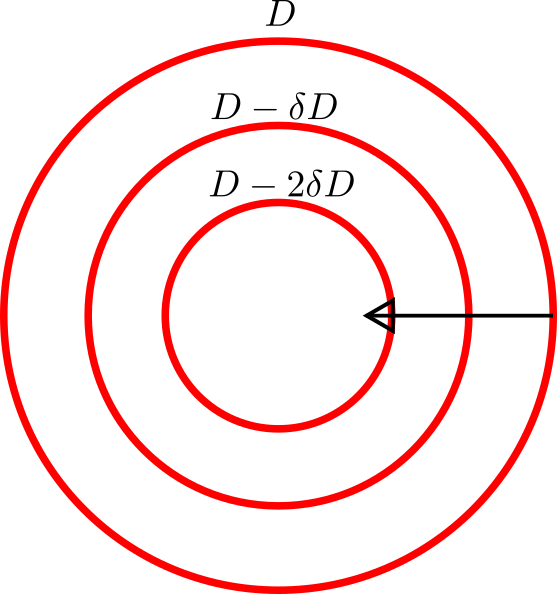
\includegraphics[width=0.7\textwidth]{figures/pms.png}
\end{figure}
\end{minipage}
\hspace*{20pt}
\begin{minipage}{0.45\textwidth}
Philosophy of Poor Man's scaling:
\begin{itemize}
	\item Successively eliminate high-energy energy shells
	\item Write high energy excitations as second-order correction to low-energy scatterings
	\item Typically perturbative
\end{itemize}
\end{minipage}
\footcite{Anderson}
}
\only<+>{
\hspace*{\fill}	\(E = \text{exact eigenvalue}\)\hspace*{\fill} \(\omega=\text{URG quantum fluctuation scale}\)\hspace*{\fill}

\vspace*{20pt}
\begin{minipage}{0.5\textwidth}
\[\Delta H_\text{PMS} = V_- \frac{1}{E - H_0}V_+ + V_+ \frac{1}{E - H_0}V_-\]
\cen{
	\large\(\Bigg\downarrow E \to \omega\)
}
\[\Delta H_\text{URG} = V_- \frac{1}{\omega - H_0}V_+ + V_+ \frac{1}{\omega - H_0}V_-\]
\end{minipage}
\begin{minipage}{0.49\textwidth}
\begin{figure}[htpb]
	\centering
	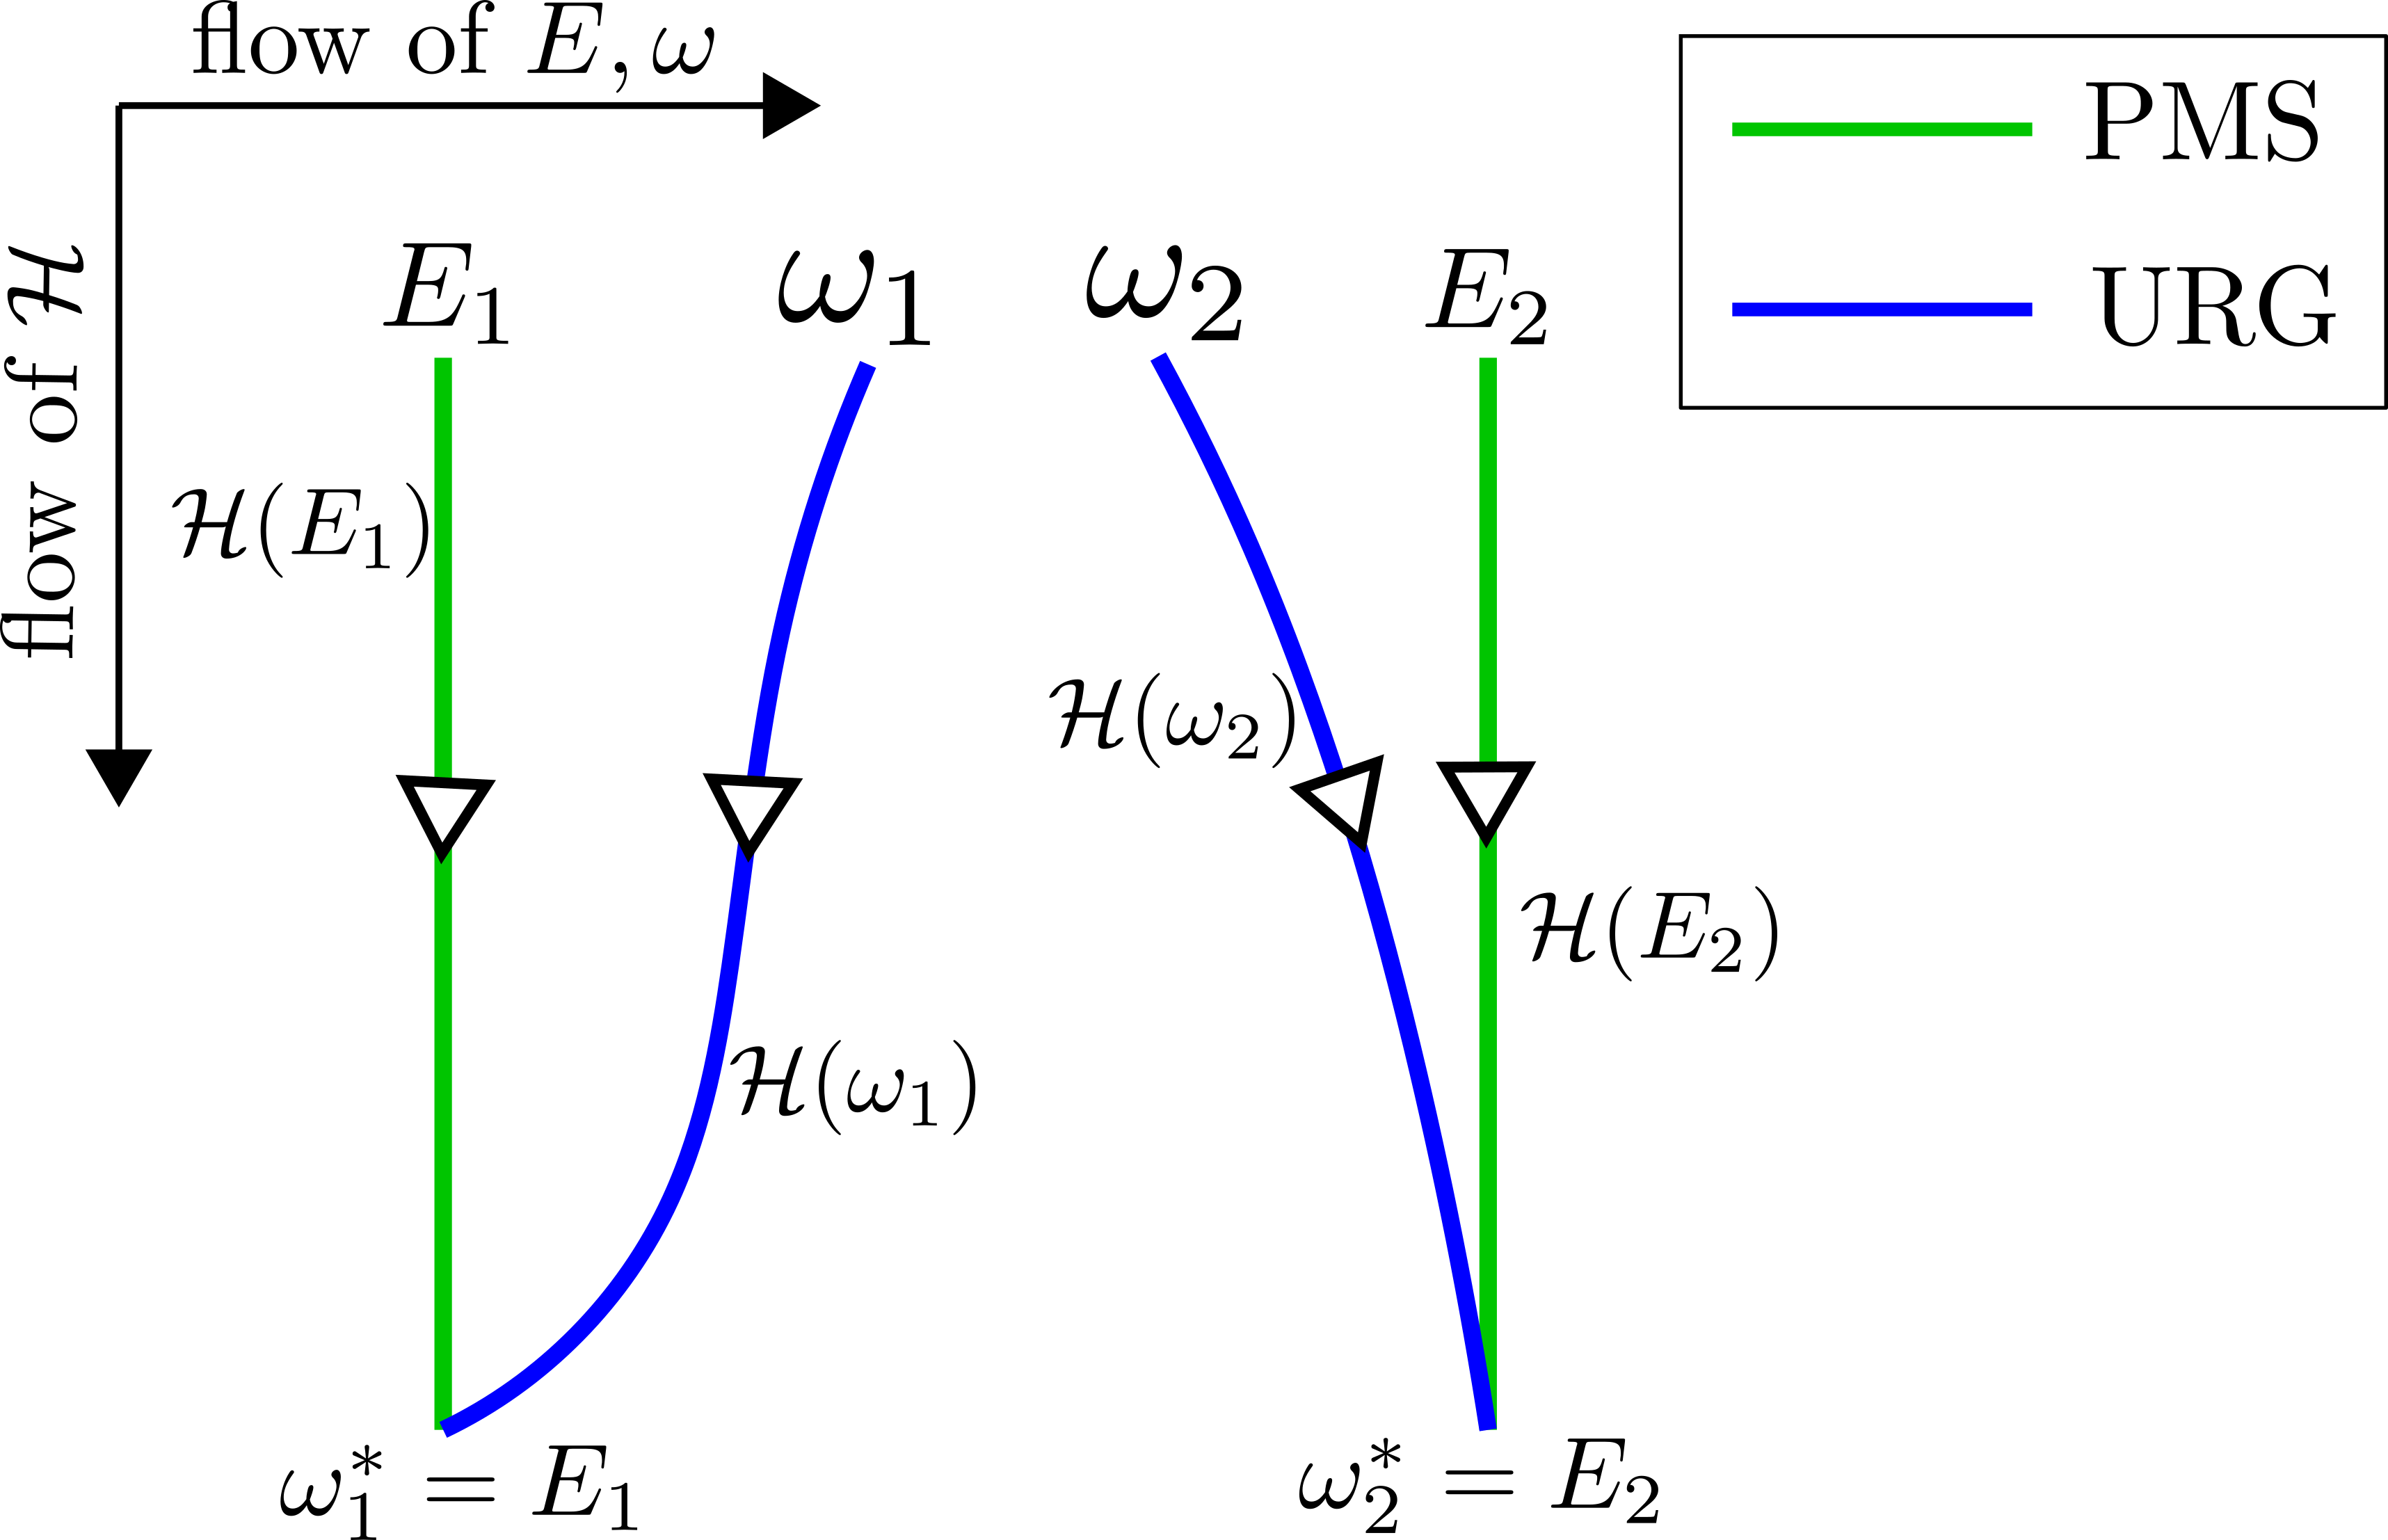
\includegraphics[width=0.9\textwidth]{figures/pms_vs_urg.png}
\end{figure}
\end{minipage}
}
\end{frame}
\begin{frame}[noframenumbering]{URG: Relation to Continuous Unitary Transformation RG}
\Large\[H = \overbrace{H_d}^\text{diagonal part} + \overbrace{H_X}^\text{off-diagonal part}\]
\cen{
	\Large$\Delta H_\text{CUT} = \Delta l\bigg[\big[H_d(l), H_X(l)\big], H(l)\bigg]$
}
\vspace*{20pt}
\only<+>{
	\begin{minipage}{0.39\textwidth}
		{\Large\(V_{kq}(l) = V_{kq}(0)e^{\left( \epsilon_k - \epsilon_q \right) l}\)}
\end{minipage}
\hspace*{0.09\textwidth}
\begin{minipage}{0.5\textwidth}
	\large{
	\begin{itemize}
		\item off-diagonal terms decay exponentially
			\vspace*{10pt}
		\item those that connect larger energy differences decay fastest
	\end{itemize}
}
\end{minipage}
\footcite{glazek-wilson,wegner_1994}
}
\only<+>{
	\vspace*{-10pt}
\cen{
	\large\(\Delta H_\text{URG} = \overbrace{\bigg[\big[H_d, \frac{1}{\omega_1 - \omega_0} \left( \hat \omega - H_d \right)^{-1} H_I\big], H\bigg]}^{\Delta H_0} - H^I\)\\[20pt]
	\large\(\Delta H_0 \xrightarrow{\left( \hat \omega - H_d \right)^{-1} \sim -H_d^{-1}} \Delta \lambda \times \bigg[\big[H_d, H_I\big], H\bigg]\)
}
}
\end{frame}
\end{document}
